%====================================================================%
%                  MORIOND.TEX                                       %
%====================================================================%

\documentclass{moriond}

\usepackage{subcaption}
\captionsetup{compatibility=false}

\bibliographystyle{unsrt}    
% for BibTeX - sorted numerical labels by order of
% first citation.

% A useful Journal macro
\def\Journal#1#2#3#4{{#1} {\bf #2}, #3 (#4)}

% Some useful journal names
\def\NCA{\em Nuovo Cimento}
\def\NIM{\em Nucl. Instrum. Methods}
\def\NIMA{{\em Nucl. Instrum. Methods} A}
\def\NPB{{\em Nucl. Phys.} B}
\def\PLB{{\em Phys. Lett.}  B}
\def\PRL{\em Phys. Rev. Lett.}
\def\PRD{{\em Phys. Rev.} D}
\def\ZPC{{\em Z. Phys.} C}

% Some other macros used in the sample text
\def\st{\scriptstyle}
\def\sst{\scriptscriptstyle}
\def\mco{\multicolumn}
\def\epp{\epsilon^{\prime}}
\def\vep{\varepsilon}
\def\ra{\rightarrow}
\def\ppg{\pi^+\pi^-\gamma}
\def\vp{{\bf p}}
\def\ko{K^0}
\def\kb{\bar{K^0}}
\def\al{\alpha}
\def\ab{\bar{\alpha}}
\def\be{\begin{equation}}
\def\ee{\end{equation}}
\def\bea{\begin{eqnarray}}
\def\eea{\end{eqnarray}}
\def\CPbar{\hbox{{\rm CP}\hskip-1.80em{/}}}
%temp replacement due to no font
%%%%%%%%%%%%%%%%%%%%%%%%%%%%%%%%%%%%%%%%%%%%%%%%%%
%                                                %
%    BEGINNING OF TEXT                           %
%                                                %
%%%%%%%%%%%%%%%%%%%%%%%%%%%%%%%%%%%%%%%%%%%%%%%%%%

%\newcommand{\Photo}{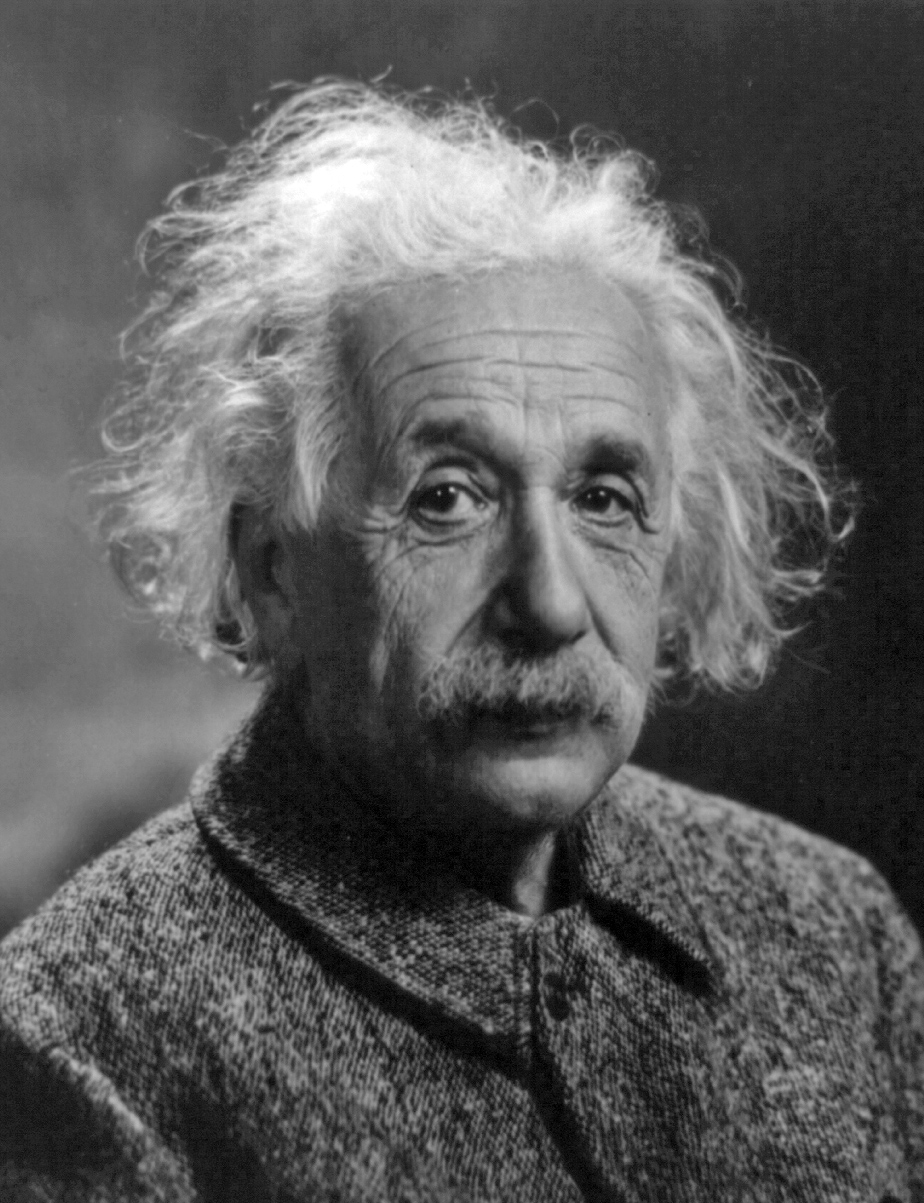
\includegraphics[height=35mm]{mypicture}}
\newcommand{\Photo}{}

\begin{document}
\title{Highlights of ATLAS Search Results}

\author{Bingxuan Liu, on behalf of the ATLAS Collaboration}

\address{Department of Physics, Simon Fraser University, Vancouver, Canada}

\maketitle\abstracts{Searching for beyond standard model (BSM) physics has been
one of the primary goals of the Large Hadron Collider (LHC).  The LHC delivered
140 $\mathrm{fb}^{-1}$ data of high quality in Run 2, allowing the ATLAS
experiment to expand and improve its search programme. The recent development
in detector performance and analysis techniques have brought significant boosts
to the search sensitivities. In this article, highlights of recent ATLAS search
results are discussed and summarised.}  

\section{Introduction}

Many mysteries in particle physics, such as the hierarchy problem, the origin
of dark matter (DM) and neutrino masses are still waiting for answers or hints
from the Large Hadron Collider (LHC). ATLAS is a general purpose detector at
the LHC that is capable of searching for beyond standard model (BSM) physics
via various approaches. ATLAS has conducted a comprehensive set of searches in
the past years. Even though no evidence of BSM physics has been reported, those
searches excluded a large part of the phase space for many models. The ATLAS
Run 2 data-taking is a great success, and a huge investment. Therefore, it is
imperative to maximise its physics return. Recent ATLAS searches are featured
with upgrading previous iterations using cutting-edge analysis techniques or
detector performance development, filling the gaps between explored regions of
phase space and considering challenging, completely uncovered signatures.      

\section{Full Run 2 Upgrades}

The detector performance in ATLAS is continuously improving, thanks to the
diligent work carried out in the relevant areas. For instance, the performance
of bottom- and top-tagging has advance significantly in the past few years. In
addition, the application of machine learning techniques have become very
mature in physics analyses, enhancing the sensitivities. Even though previous
analyses have explored similar final states, taking advantage of the above
facts and more data, the full Run 2 upgrades of those searches will push
the exclusion limits further.\\

In the full Run 2 ATLAS vector-like quark search, the top partner masses with
50\% decay width are excluded up to 1975 GeV for the singlet representation,
considering $B(T\rightarrow Wb)=0.5$, as shown in
Figure~\ref{fig:limits1}\subref{fig:vlq}. Compared to the previous analysis
probing the same final state, this analysis adopted an updated top-tagger and
more optimised selections, achieving greatly improved sensitivities~\cite{vlq}. The
ATLAS full Run 2 right-handed neutrino search sets the most stringent limits on
the Keung-Senjanovi\'c process in the TeV $W$ partner ($W_{\mathrm{R}}$) mass
region. This search considers both the ``resolved'' and ``merged'' cases,
depending on the mass split between the $W_{\mathrm{R}}$ and the heavy neutrino
($N_{\mathrm{R}}$). For Majorana neutrinos, in the muon channel, the limit on
$m(W_{\mathrm{R}})$ reaches 6.4 TeV for $m(N_{\mathrm{R}})=1$ TeV, and the
limit on $m(N_{\mathrm{R}})$ extends to 3.6 TeV for $m(W_{\mathrm{R}})=4.8$
TeV, as shown in Figure~\ref{fig:limits1}\subref{fig:rhn}~\cite{rhn}.\\           

Combination of different analyses offers a powerful way to constrain a given
type of model. A recent ATLAS search is concentrated on final states with $\tau$ leptons
and hadronic jets, providing interpretation including both the leptoquark and
excited $\tau$ models. In particular, it is sensitive to $LQ\rightarrow
c\tau^{-}$ ($\overline{LQ}\rightarrow\overline{c}\tau^{+}$) decays, as the
analysis does not enforce any jets to be $b$-tagged. It comprises a critical
piece in the leptoquark combination given this unique feature of the signal
region selection. As seen in Figure~\ref{fig:limits1}\subref{fig:excited},
$LQ$ masses below 1.3 TeV are excluded, assuming the branching ratio of their
decays to the $c$-quark–$\tau$-lepton pair is equal to one~\cite{tau}.\\   


\begin{figure}[htp]
     \centering
     \begin{subfigure}[b]{0.35\textwidth}
         \centering
         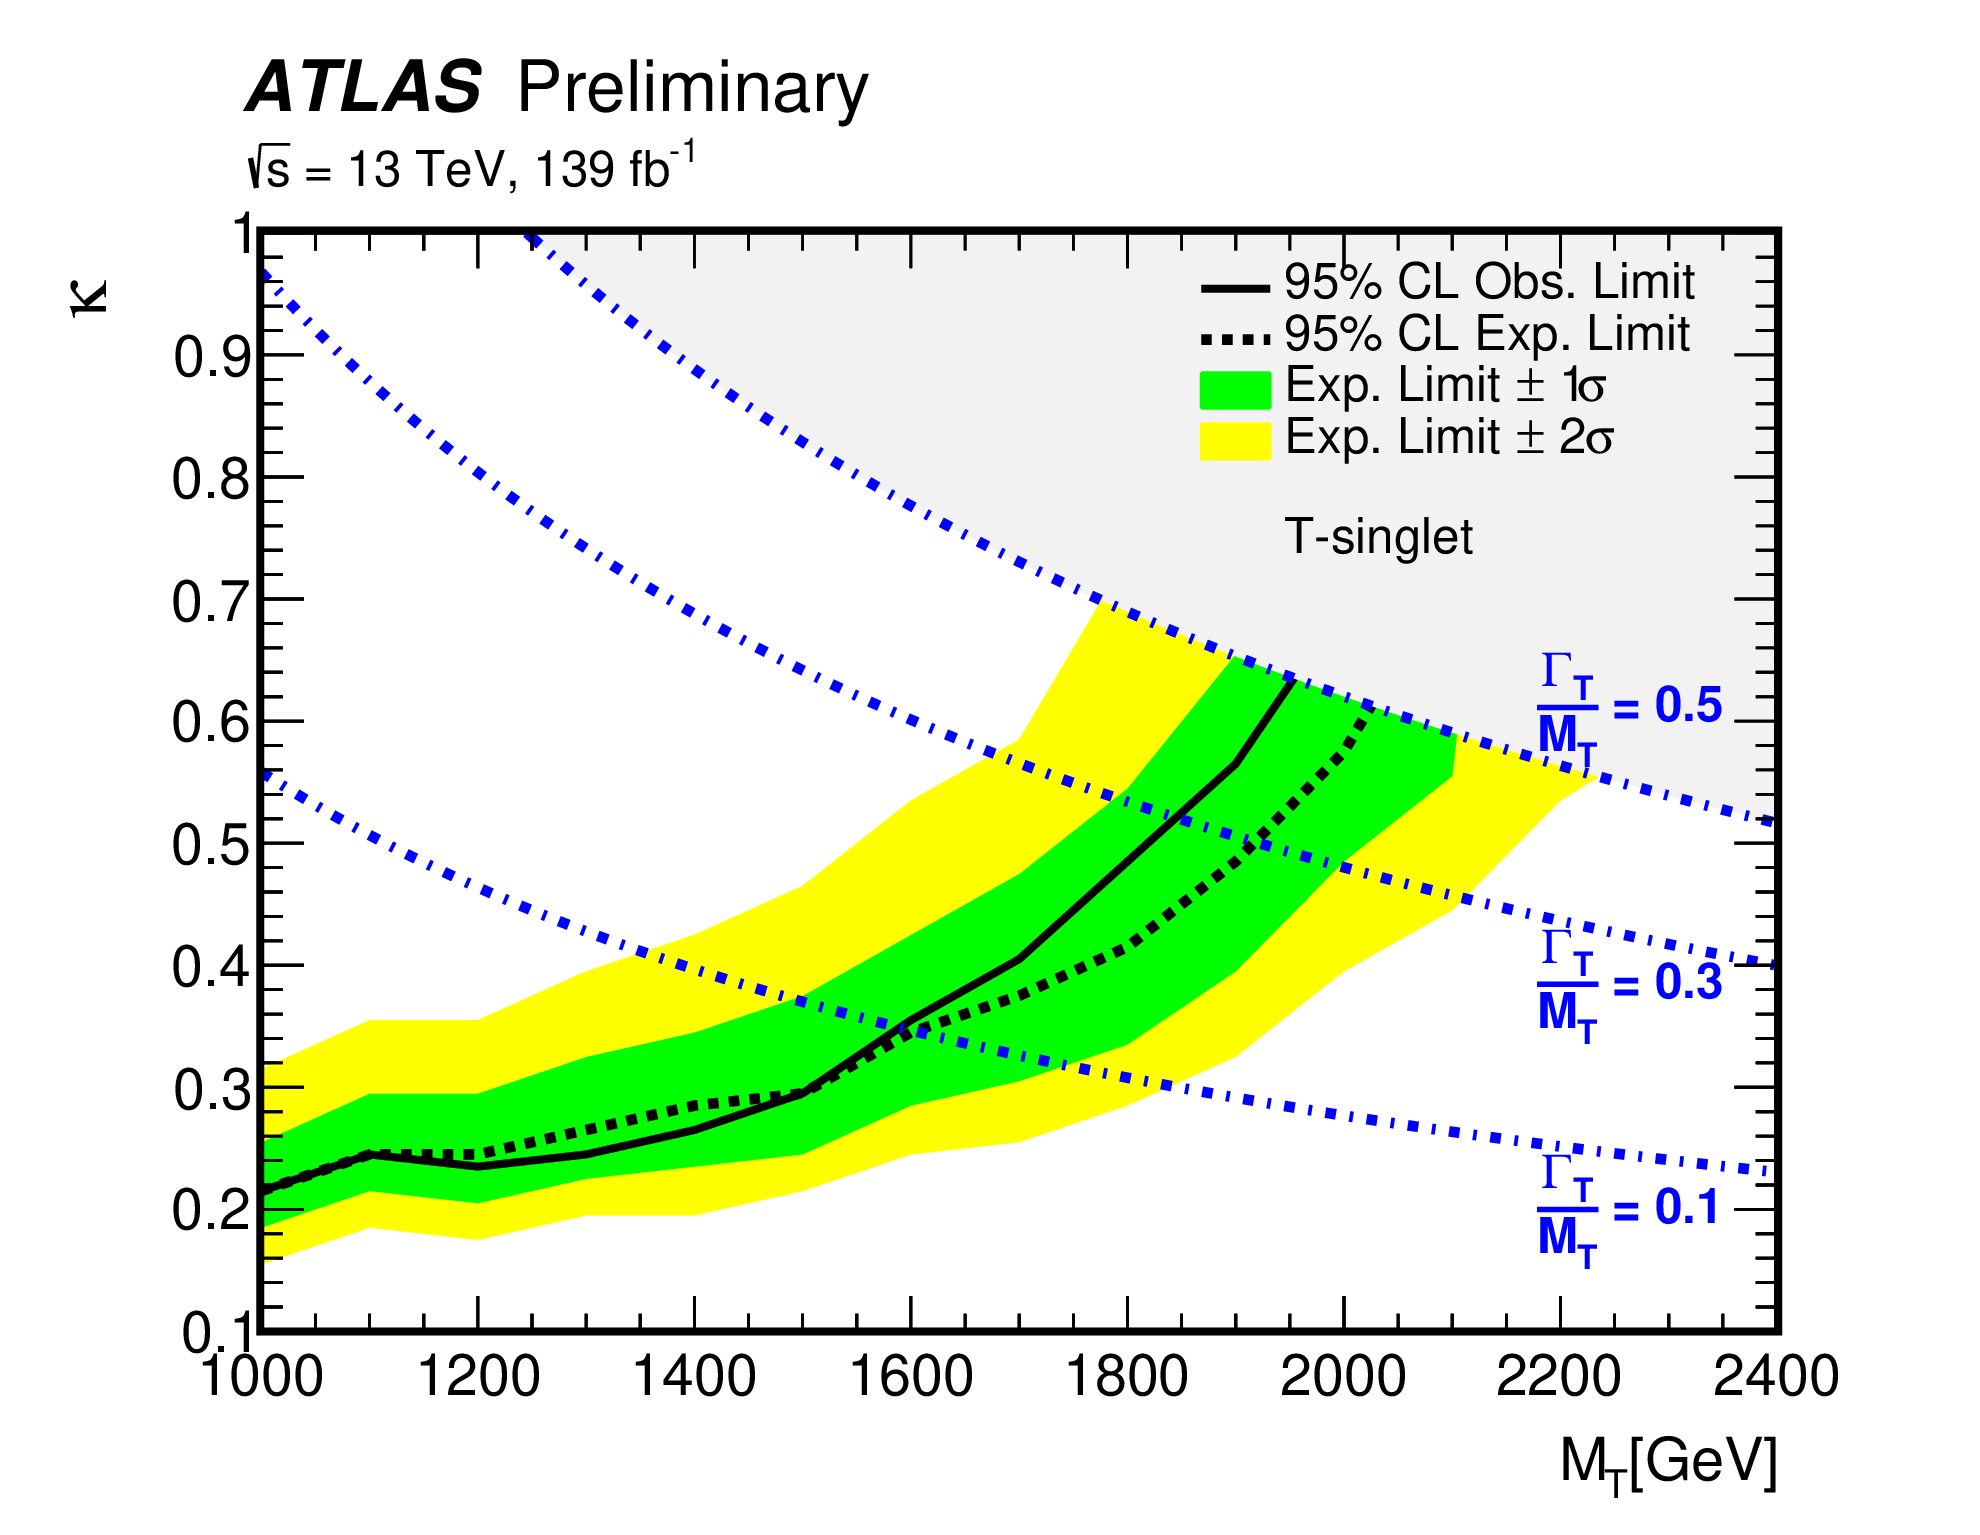
\includegraphics[width=\textwidth]{VLQ}
         \caption{}
         \label{fig:vlq}
     \end{subfigure}
     \begin{subfigure}[b]{0.30\textwidth}
         \centering
         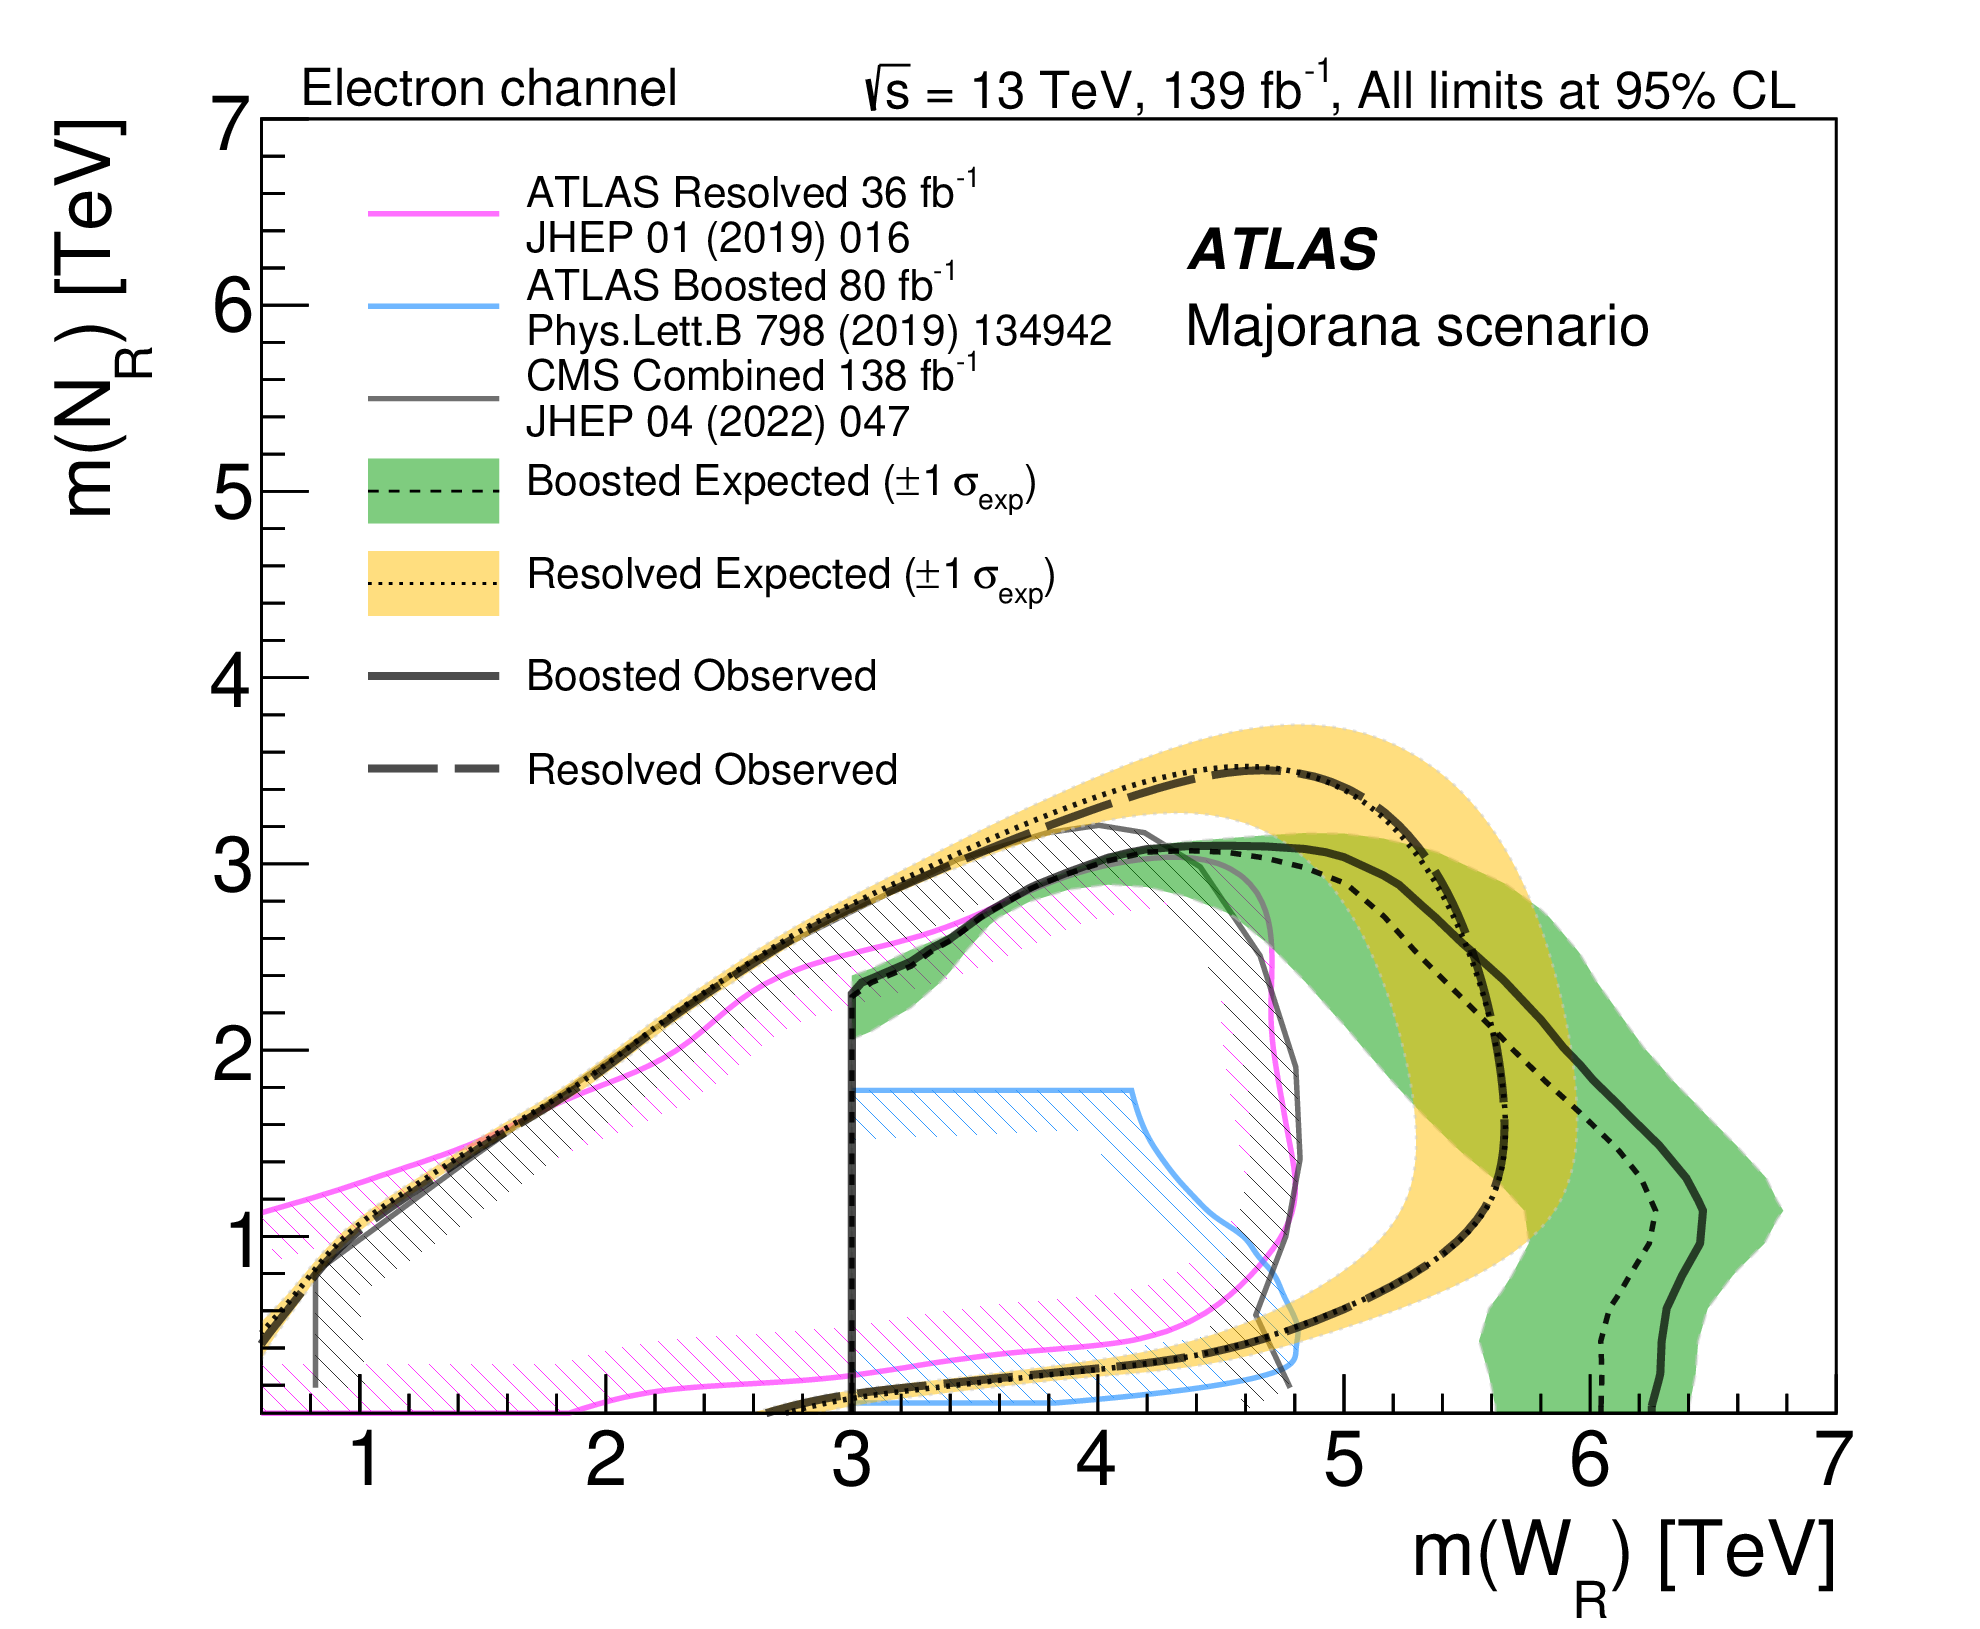
\includegraphics[width=\textwidth]{RHN}
         \caption{}
         \label{fig:rhn}
     \end{subfigure}
     \begin{subfigure}[b]{0.25\textwidth}
         \centering
         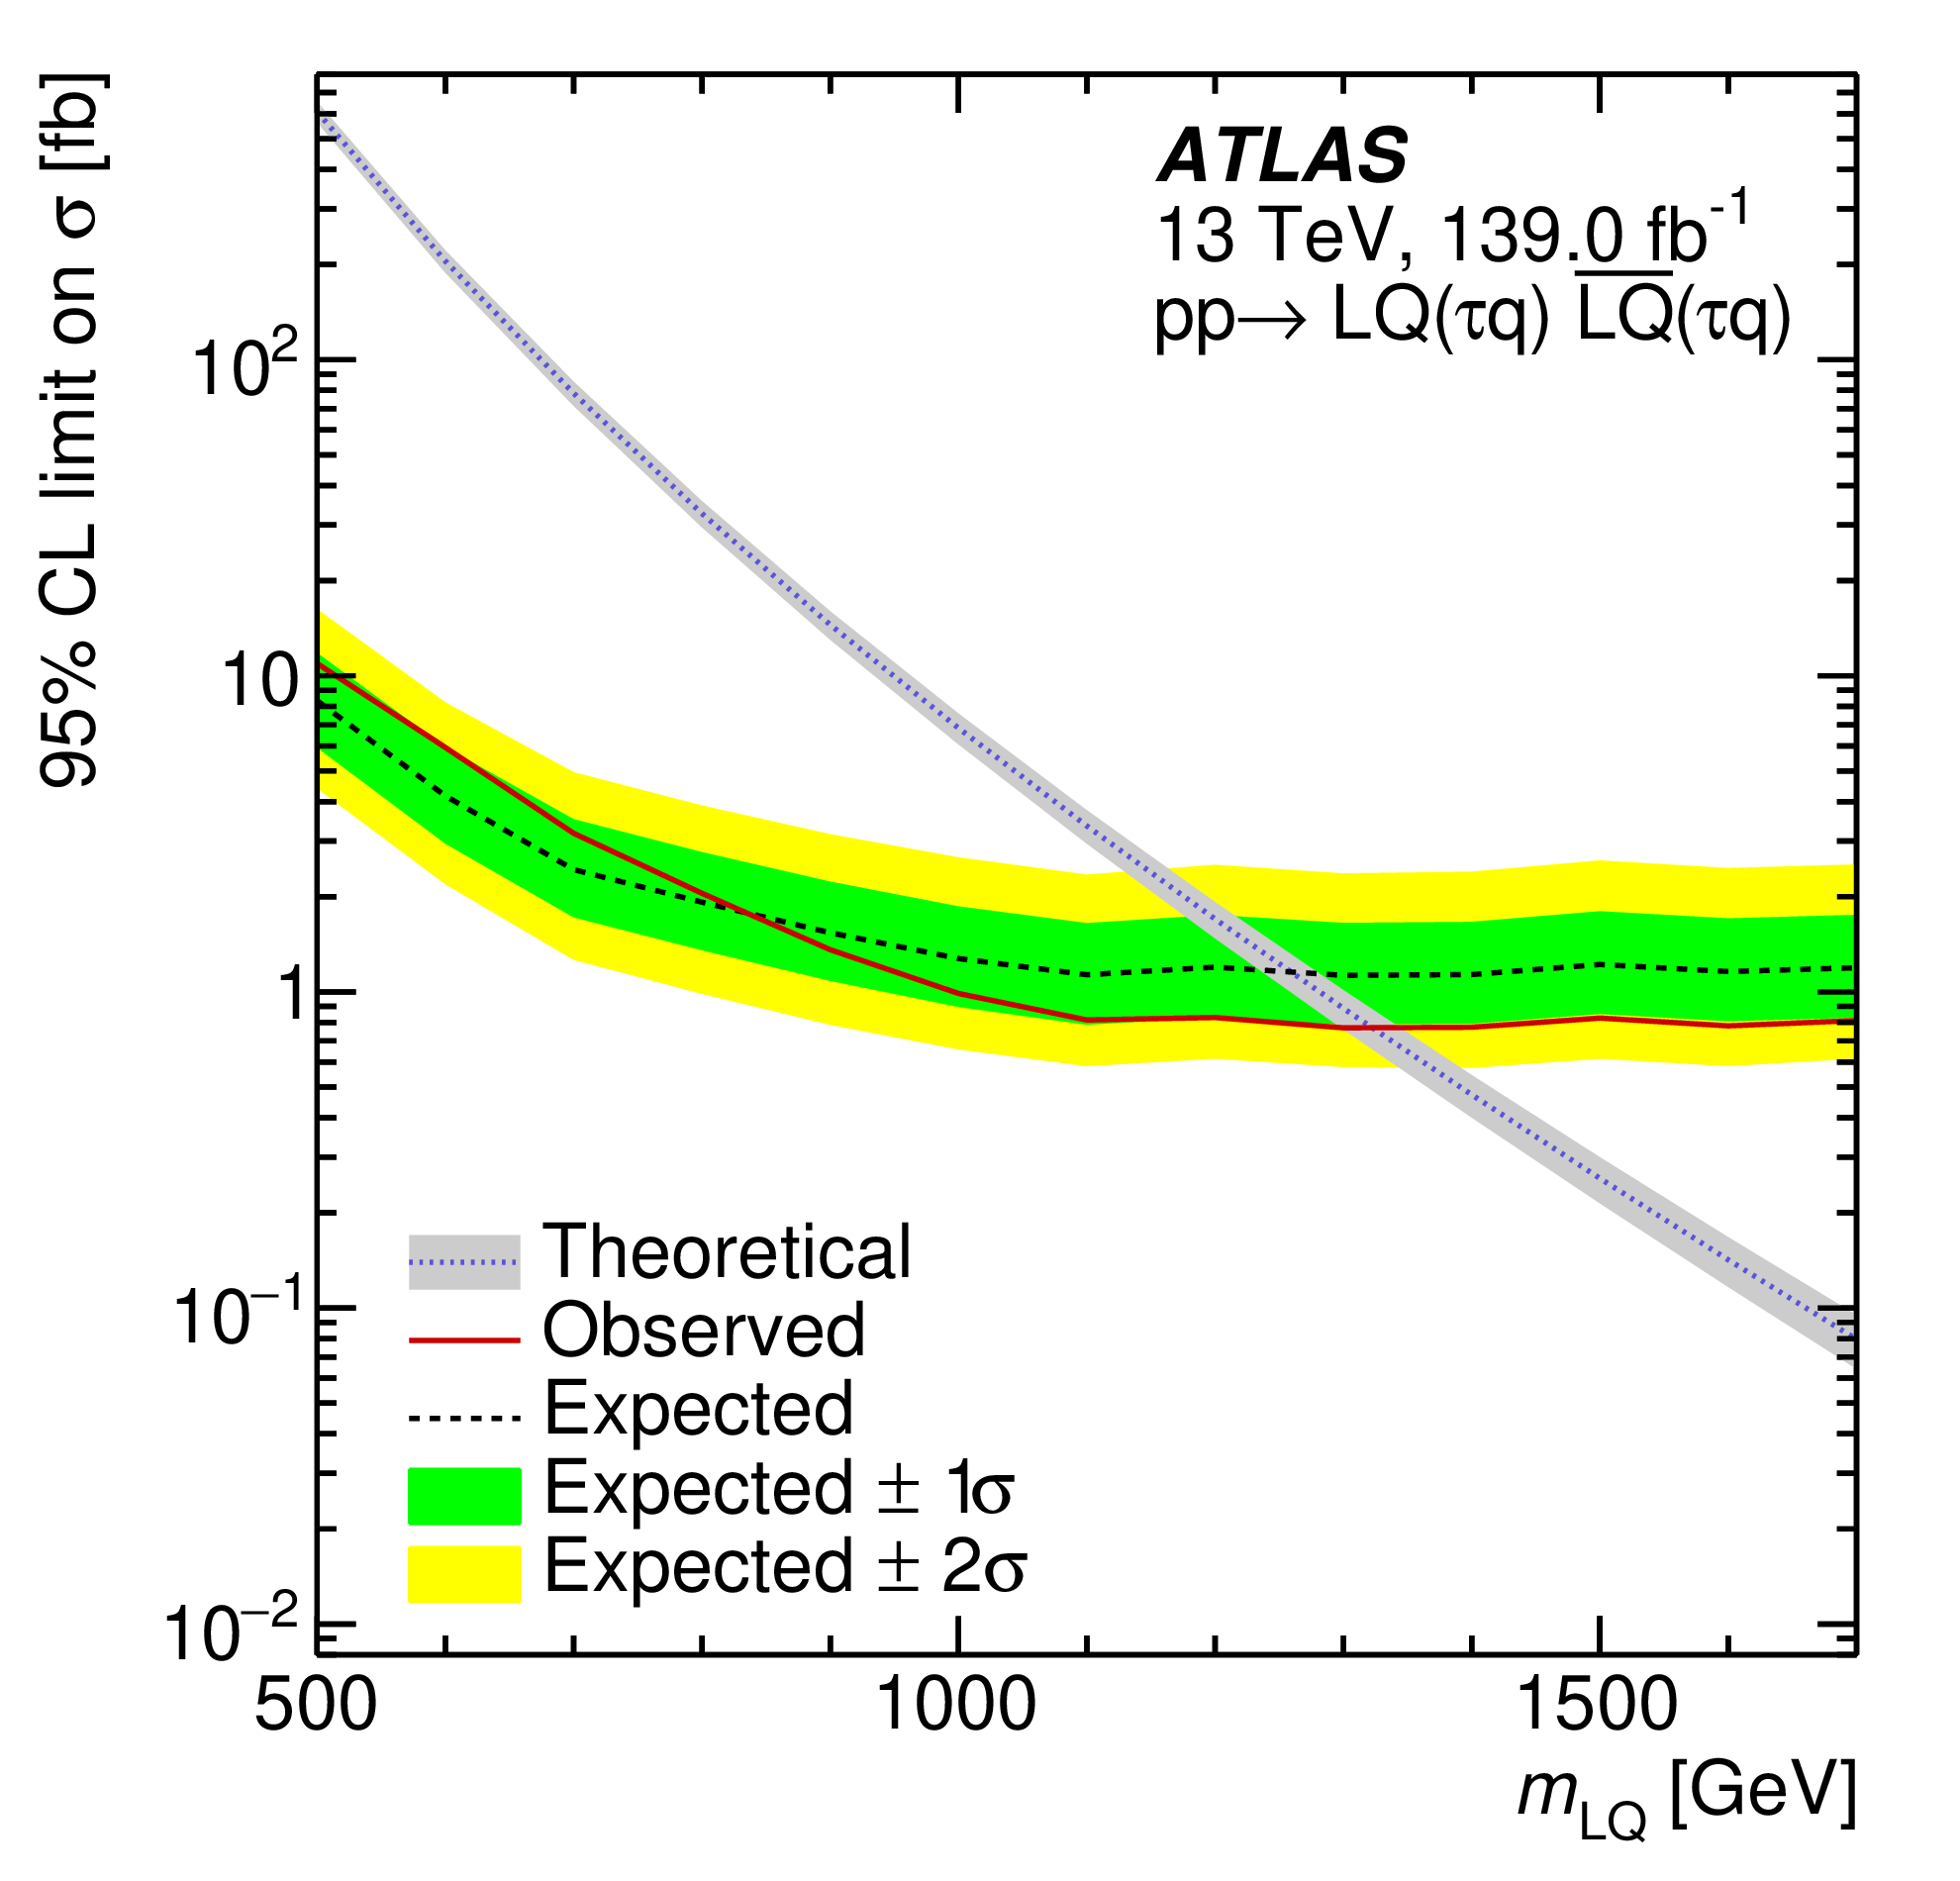
\includegraphics[width=\textwidth]{excited}
         \caption{}
         \label{fig:excited}
     \end{subfigure}
     \caption{(a): Observed (solid line) and expected (dashed line) limits on the singlet representation of a vector like top-quark\protect\cite{vlq}. (b): Exclusion contour of the Majorana heavy neutrino on the $m(W_{\mathrm{R}})-m(N_{\mathrm{R}})$ mass plane\protect\cite{rhn}. (c): Observed (solid line) and expected (dashed line) limits on LQ pair production where the LQ decays to a $\tau$ lepton and a charm quark\protect\cite{tau}.}
     \label{fig:limits1}
\end{figure}

\section{Filling the Gap}

There have been many BSM models proposed by the theory community in the past
decades. The number of free parameters in those models can be so large that
a single search can only probe a subset of the parameter space, a particular
combination of masses and couplings. Naturally, there are gaps between existing
searches, and they need to be explored. The gap regions are usually hard to
study so that special analysis strategies are essential.\\

Supersymmetry has been searched extensively at the LHC by a comprehensive
programme. However various uncovered corners have been present on specific
parameter planes. A recent ATLAS search for higgsinos considers the
$b\overline{b}\gamma\gamma$ final state, taking advantage of the excellent mass
resolution of the photons and the large $H\rightarrow b\overline{b}$ branching
ratio. It successfully fills the gap in the low mass region, as seen in Figure
~\ref{fig:limits2}\subref{fig:bbyy}~\cite{bbyy}.\\

The gap between dedicated long-lived particle (LLP) searches and conventional
searches is becoming increasingly important. A recent ATLAS search for
micro-displaced muons is focused on this region using muons reconstructed by the
standard algorithms, requiring the impact parameter ($|d_{0}|$) of the muons to
be between 0.1 and 3 mm. Control regions, validation regions, and signal
regions are constructed using the muon $|d_{0}|$ and muon-pair mass. In the
context of a smuon pair production, the smuon lifetimes down to 1 $ps$ and
smuon masses up to 520 GeV are excluded, as shown in Figure
~\ref{fig:limits2}\subref{fig:micro}~\cite{micro}.\\   

Searching for BSM is a primary goal for many experiments. It is pivotal to make
the most of LHC's higher collision energy and large integrated luminosity, in
order to complete the picture. A recent ATLAS search looks for dark photons in
the 4$l$ + $X$ final state, where the four leptons are from two dark photons
($A'$). The average invariant mass of the two lepton pairs is used as the main
observable. The four lepton mass is used to construct signal and control
regions, while the lepton pair mass is used to suppress quarkonia background.
This search excludes a much wider mass region compared to the results from the
Belle collaboration, as shown in Figure
~\ref{fig:limits2}\subref{fig:dark}~\cite{dark}.\\ 

\clearpage

\begin{figure}[htp]
     \centering
     \begin{subfigure}[b]{0.24\textwidth}
         \centering
         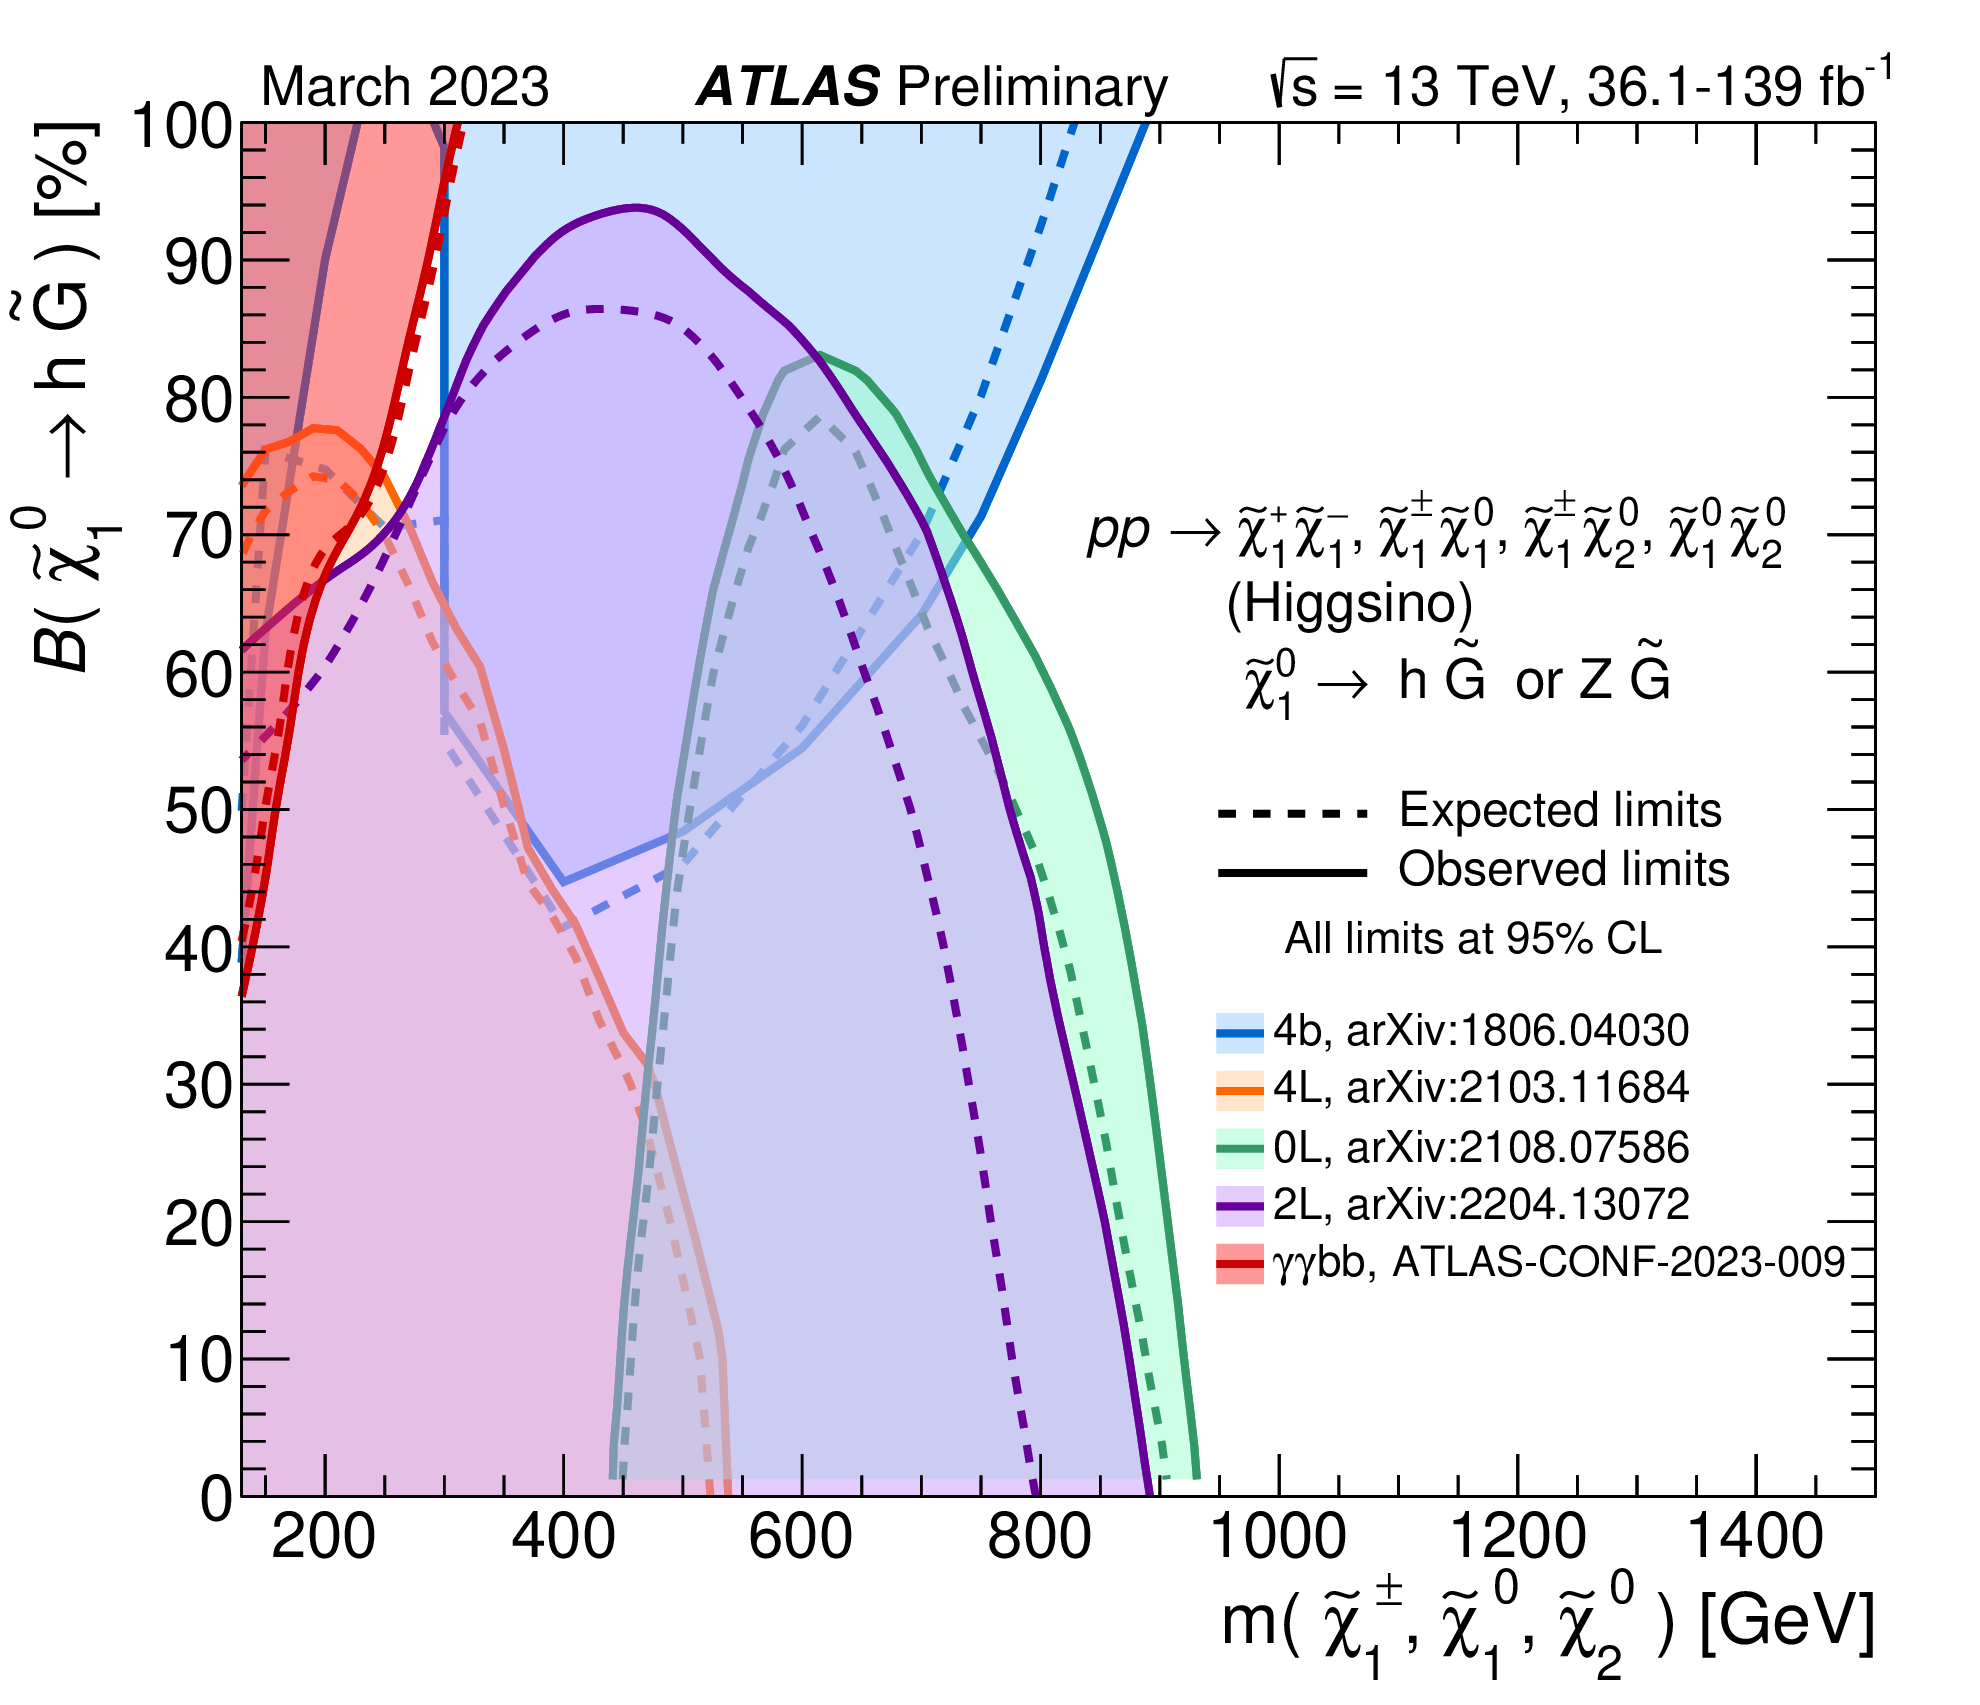
\includegraphics[width=\textwidth]{bbyy}
         \caption{}
         \label{fig:bbyy}
     \end{subfigure}
     \begin{subfigure}[b]{0.22\textwidth}
         \centering
         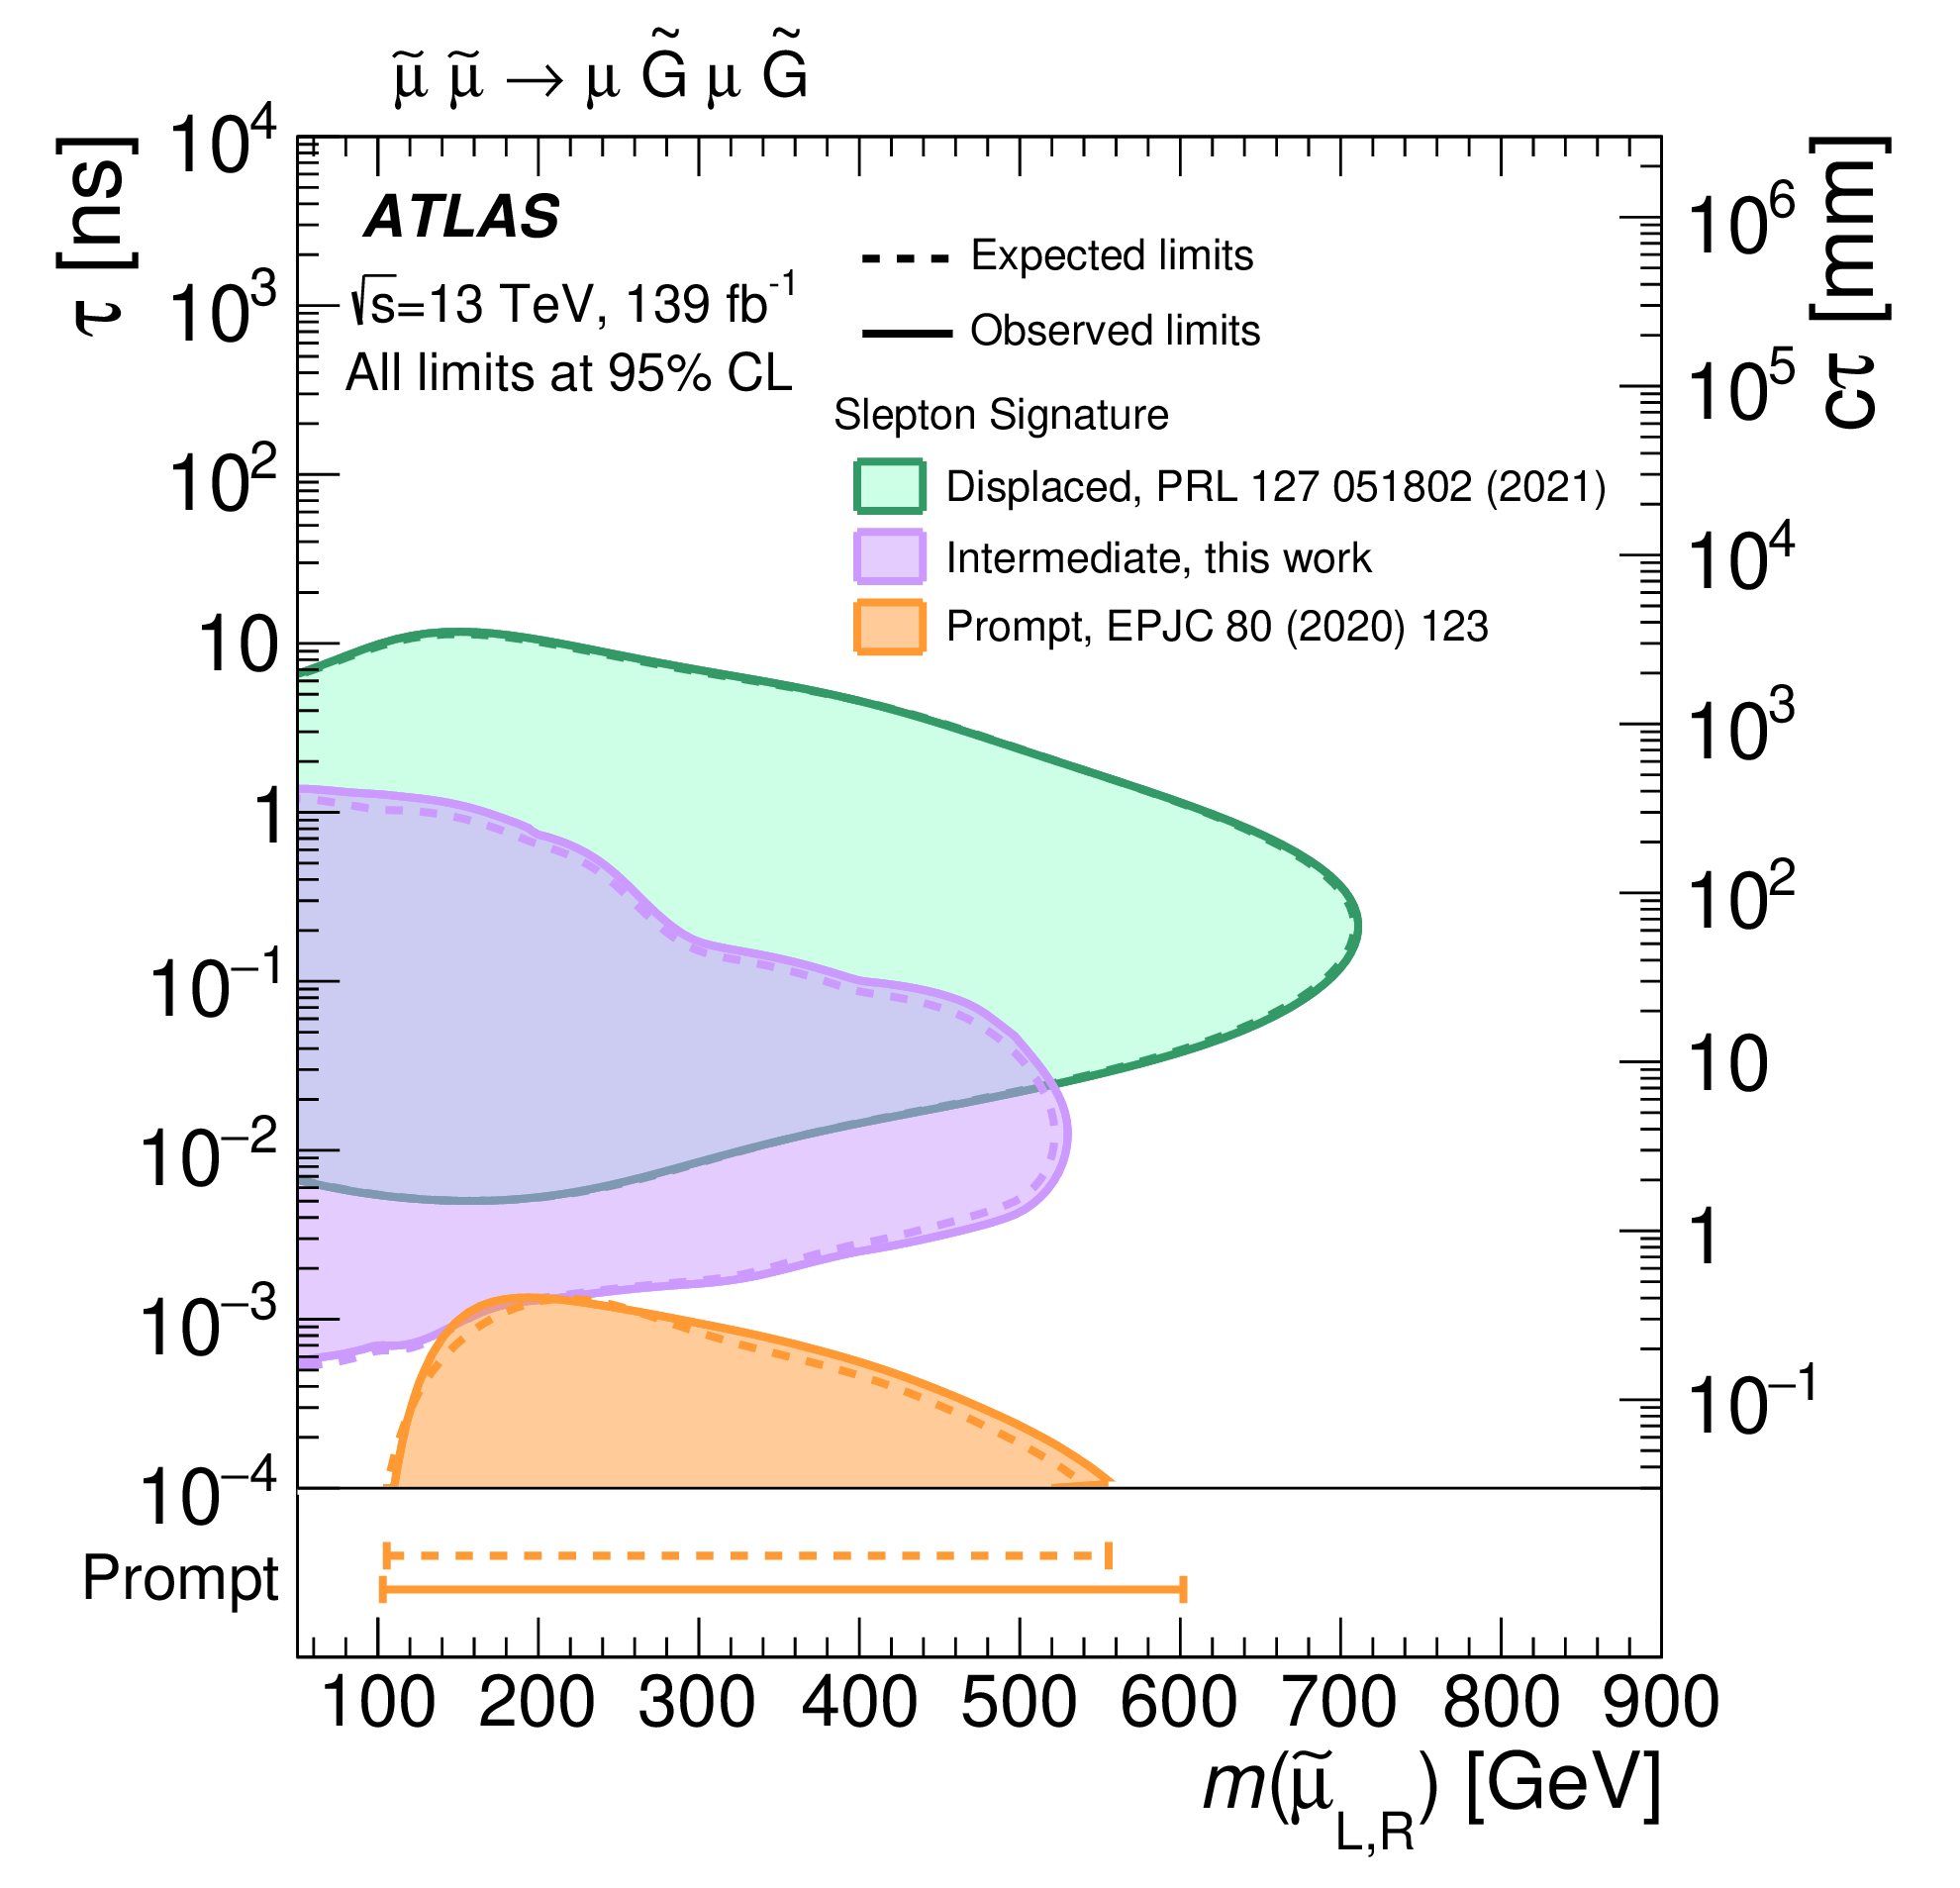
\includegraphics[width=\textwidth]{micro}
         \caption{}
         \label{fig:micro}
     \end{subfigure}
     \begin{subfigure}[b]{0.28\textwidth}
         \centering
         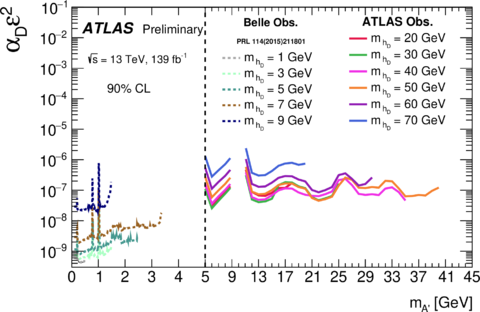
\includegraphics[width=\textwidth]{dark}
         \caption{}
         \label{fig:dark}
     \end{subfigure}
        \caption{(a): Exclusion contour of the higgsino pair production on the mass and branching ratio 2D plane\protect\cite{bbyy}. (b): Exclusion contour of the smuon pair production on the mass and lifetime 2D plane\protect\cite{micro}. (c): Exclusion limits on the dark sector couplings as a function of dark photon mass\protect\cite{dark}.}
        \label{fig:limits2}
\end{figure}

\section{New and Challenging Signatures}

ATLAS is capable of studying an impressive amount of signatures, but there are
signatures known to be very challenging. For instance, searches for LLPs
usually need to develop dedicated triggering or reconstruction algorithms.
Besides less optimal detector performance in certain regions, a signature can
be strenuous because the traditional analysis techniques are not suitable.
Analyses challenging those signatures can greatly broaden the ATLAS search
programme.\\

ATLAS has searched for heavy particles produced in association with two
top-quarks, decaying to two top-quarks, i.e., top-philic heavy particles. The
previous search considered the non-resonant production as the reconstructed
$t\overline{t}$ mass is very broad as seen in
Figure~\ref{fig:tttt}\subref{fig:mass}. A recent ATLAS analysis takes the
resonant production channel into account. A hybrid background estimation method
is developed to overcome the difficulties in dealing with broad signals. A
background template is obtained in an inclusive region first and then
propagated to the signal region via simulation, in order to minimize the biases
introduced by the broad signals. A global deviation scan is done first in a
model agnostic way, observing no significant deviations from the background in
data, presented in Figure~\ref{fig:tttt}\subref{fig:bump}. The observed
(expected) limits range from 21 (14) fb to 119 (86) fb depending on the choice
of model parameters, shown in Figure~\ref{fig:tttt}\subref{fig:ttttlimits}. The
results are limited by the modeling uncertainties~\cite{tttt}.\\    

\begin{figure}[htp]
     \centering
     \begin{subfigure}[b]{0.28\textwidth}
         \centering
         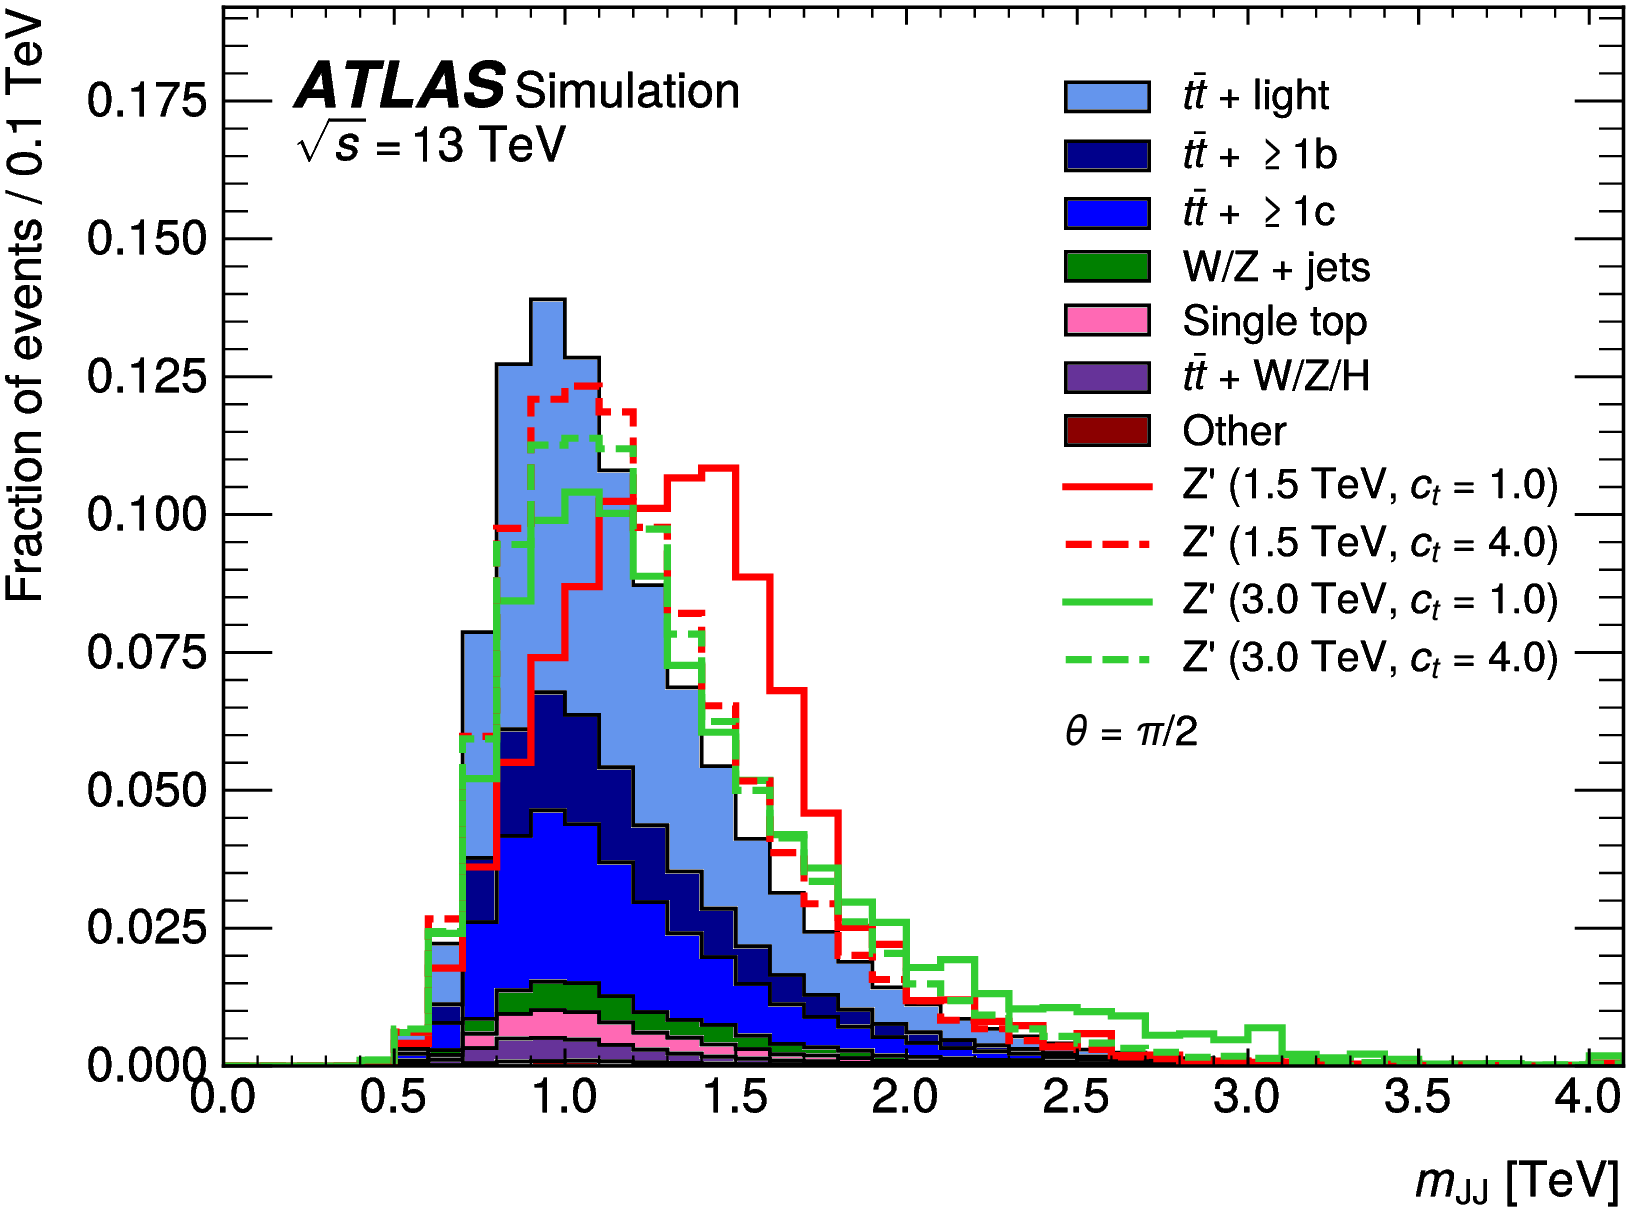
\includegraphics[width=\textwidth]{mass}
         \caption{}
         \label{fig:mass}
     \end{subfigure}
     \begin{subfigure}[b]{0.21\textwidth}
         \centering
         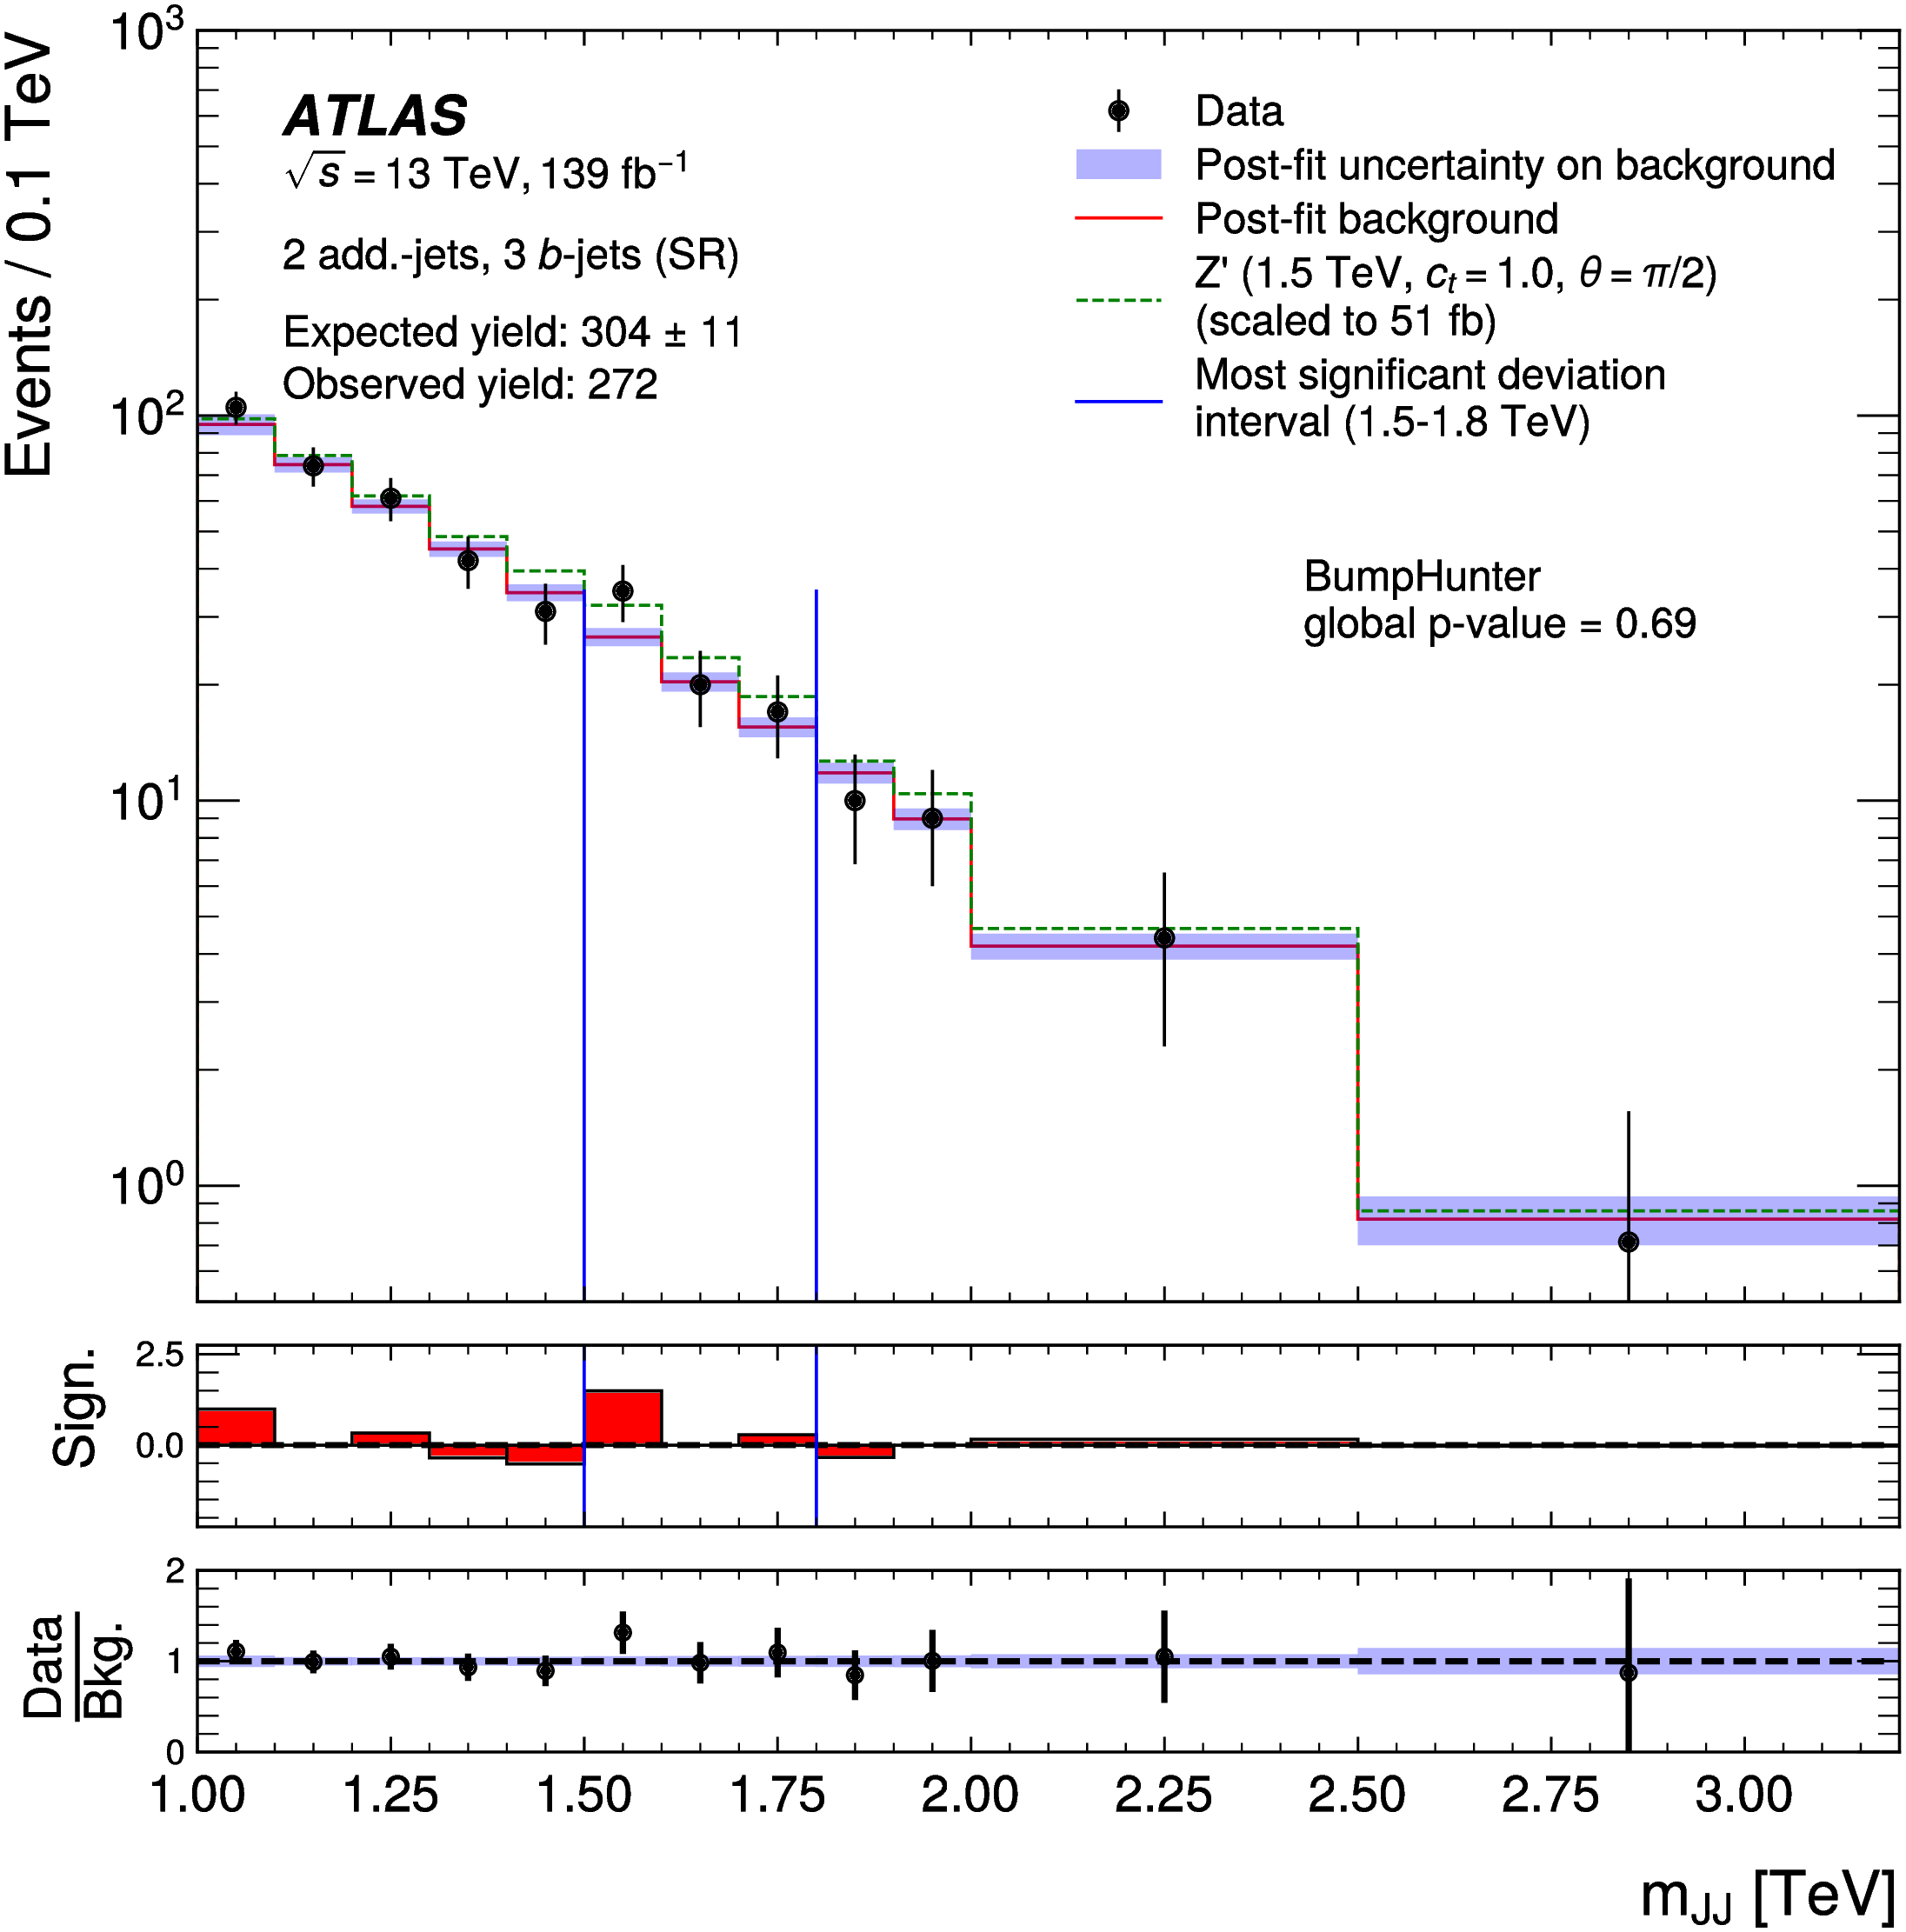
\includegraphics[width=\textwidth]{bump}
         \caption{}
         \label{fig:bump}
     \end{subfigure}
     \begin{subfigure}[b]{0.23\textwidth}
         \centering
         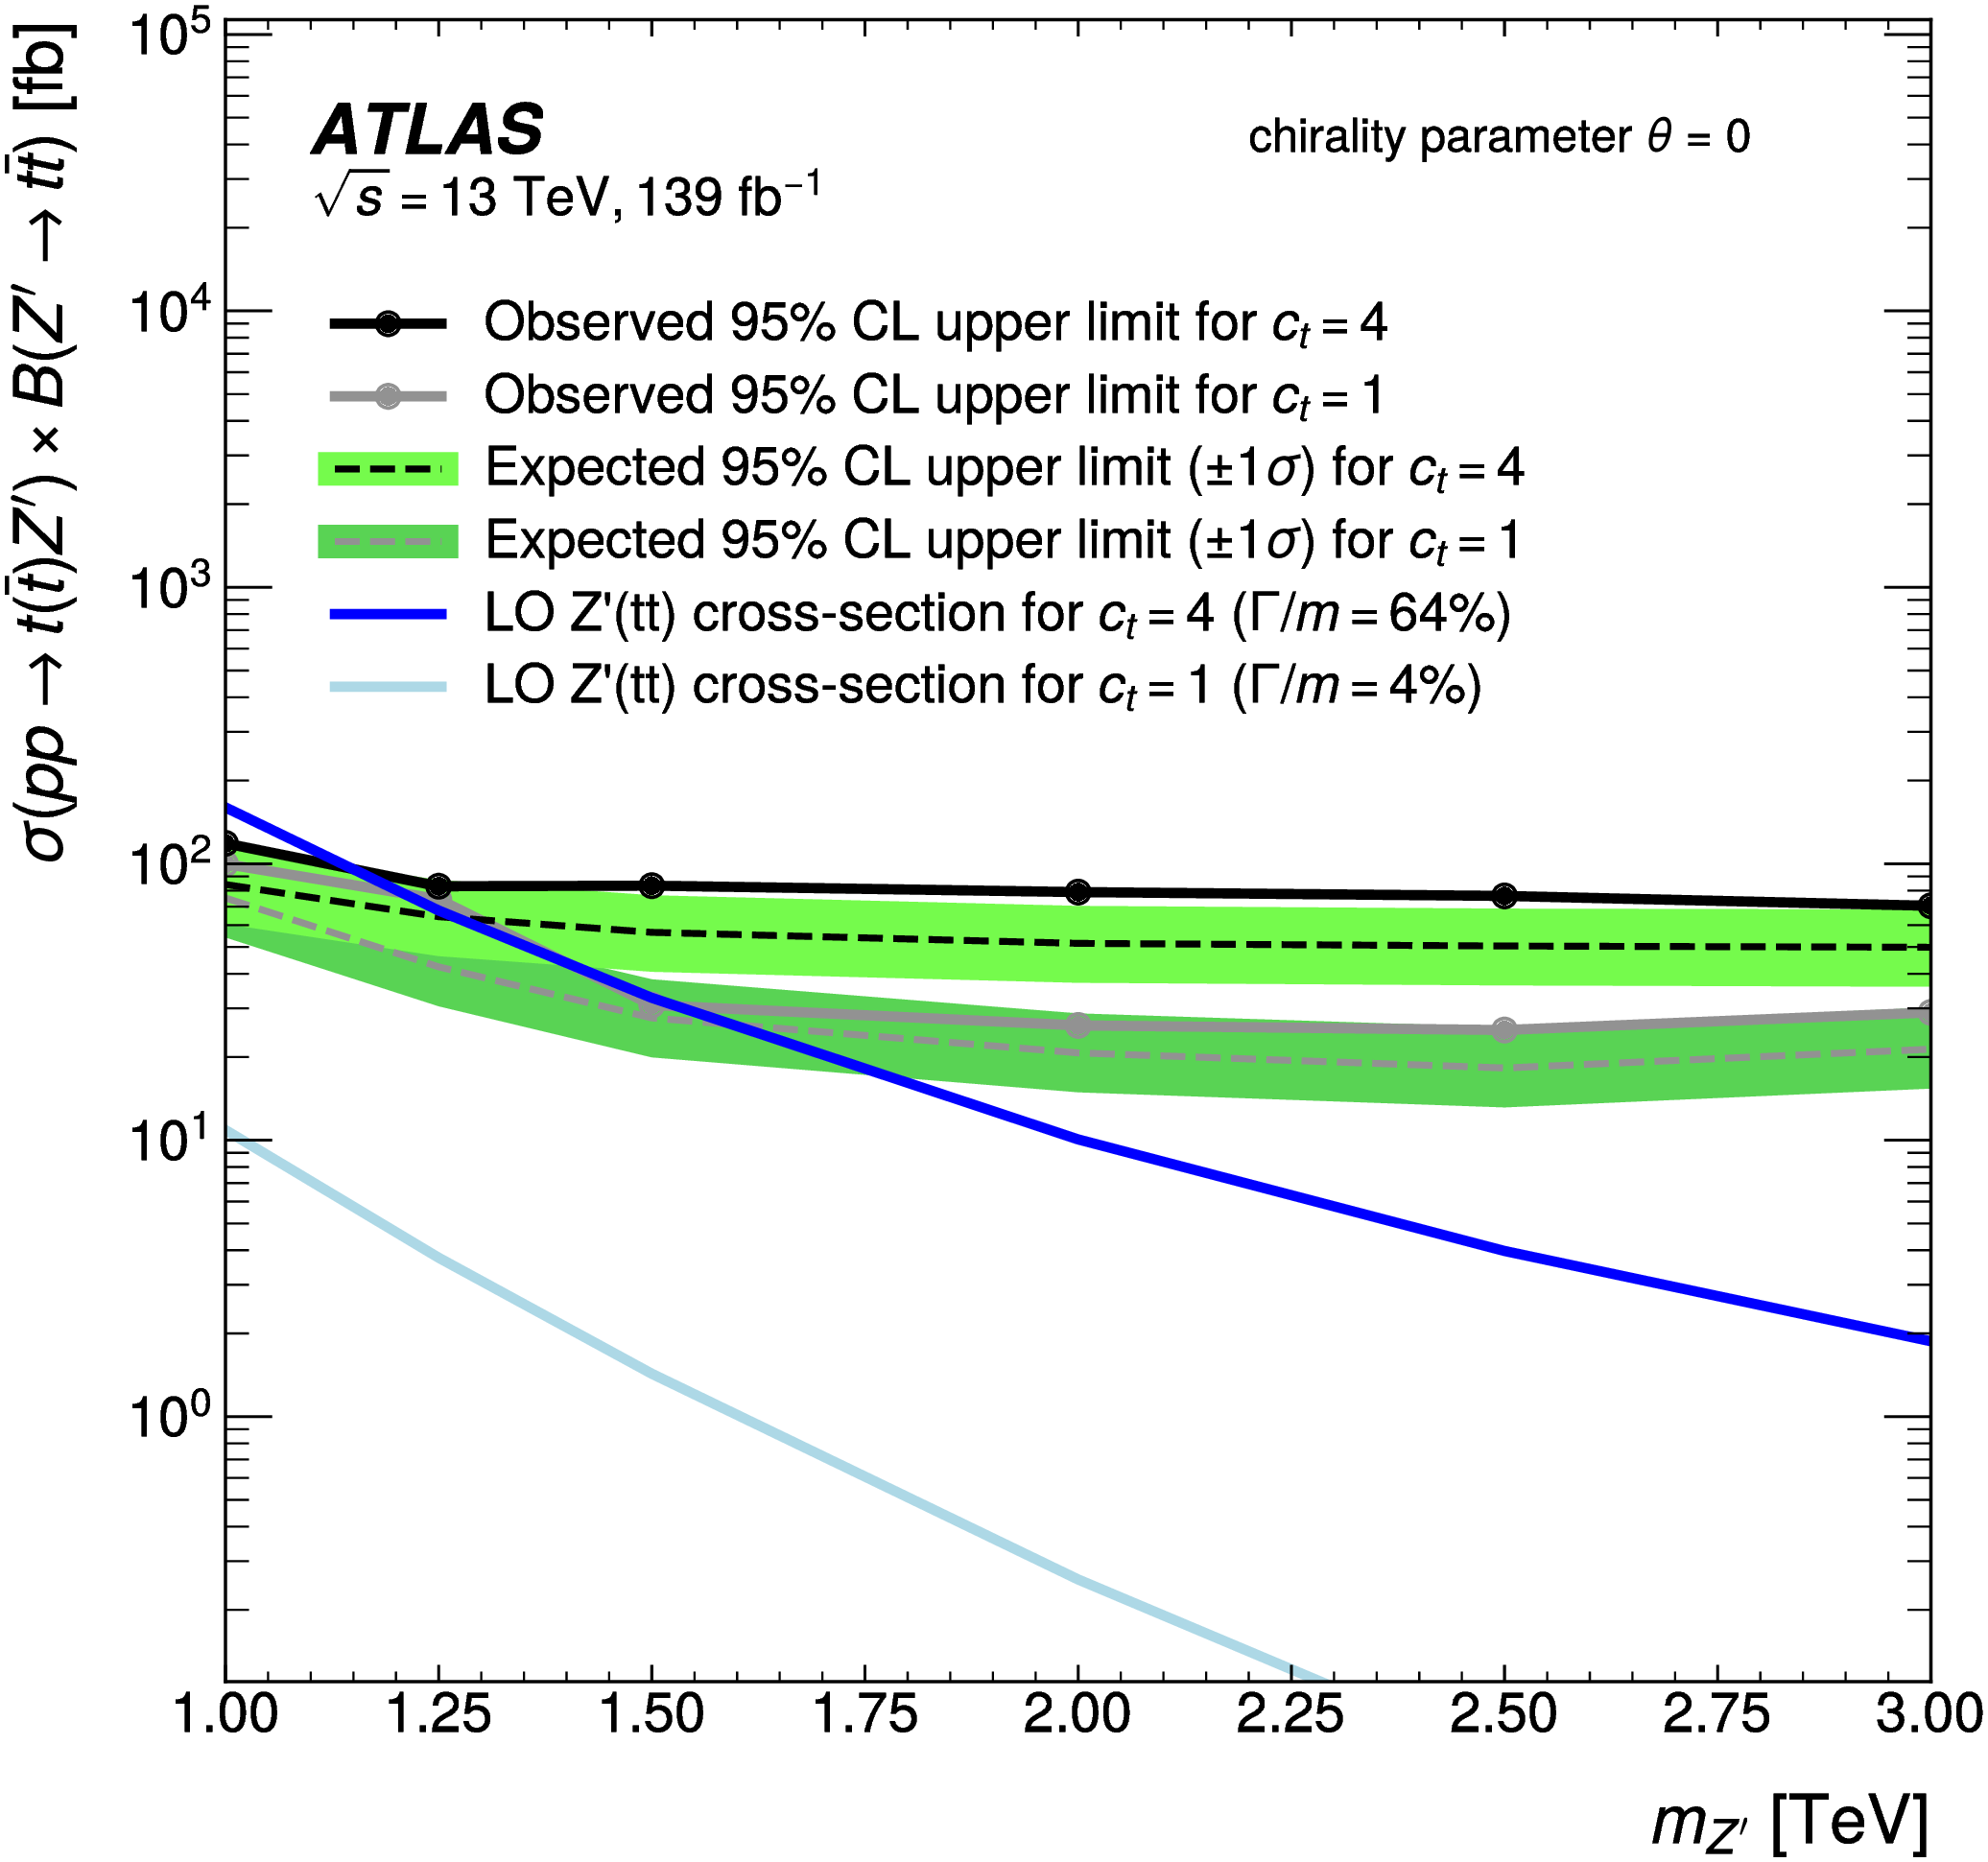
\includegraphics[width=\textwidth]{tttt}
         \caption{}
         \label{fig:ttttlimits}
     \end{subfigure}
        \caption{(a): Invariant mass distributions of the two large-R jets for different backgrounds and signal points. (b): Global deviation scan of the invariant mass spectrum. No significant deviations are observed. (c): Observed (solid line) and expected (dashed line) limits on the top-philic heavy particles as a function of mass\protect\cite{tttt}.}
        \label{fig:tttt}
\end{figure}

Searches are typically performed using intuitive observables such as the
invariant mass as the one discussed above. A recent ATLAS search explores
periodic signals for the first time. Such a signal is predicted in the
ClockWork (CW) or LinearDilation (LD) framework. Instead of having one peak in
the invariant mass spectrum, a periodic signal predicts continuous narrow
peaks, as illustrated in Figure~\ref{fig:periodic}\subref{fig:signal}. The analysis applied a
``continuous wavelet'' transformation to separate the signal events from the
background in a scalogram more efficiently, depicted in Figure
~\ref{fig:periodic}\subref{fig:shape}. Limits are set for the gravity scale, $M_{5}$, and the
turn-on mass scale, $k$, shown in Figure ~\ref{fig:periodic}\subref{fig:perlimits}~\cite{period}.
This search has not only pioneered this intriguing signature, but also
demonstrated that the data can be analyzed in a non-traditional space.\\        

\begin{figure}[htp]
     \centering
     \begin{subfigure}[b]{0.25\textwidth}
         \centering
         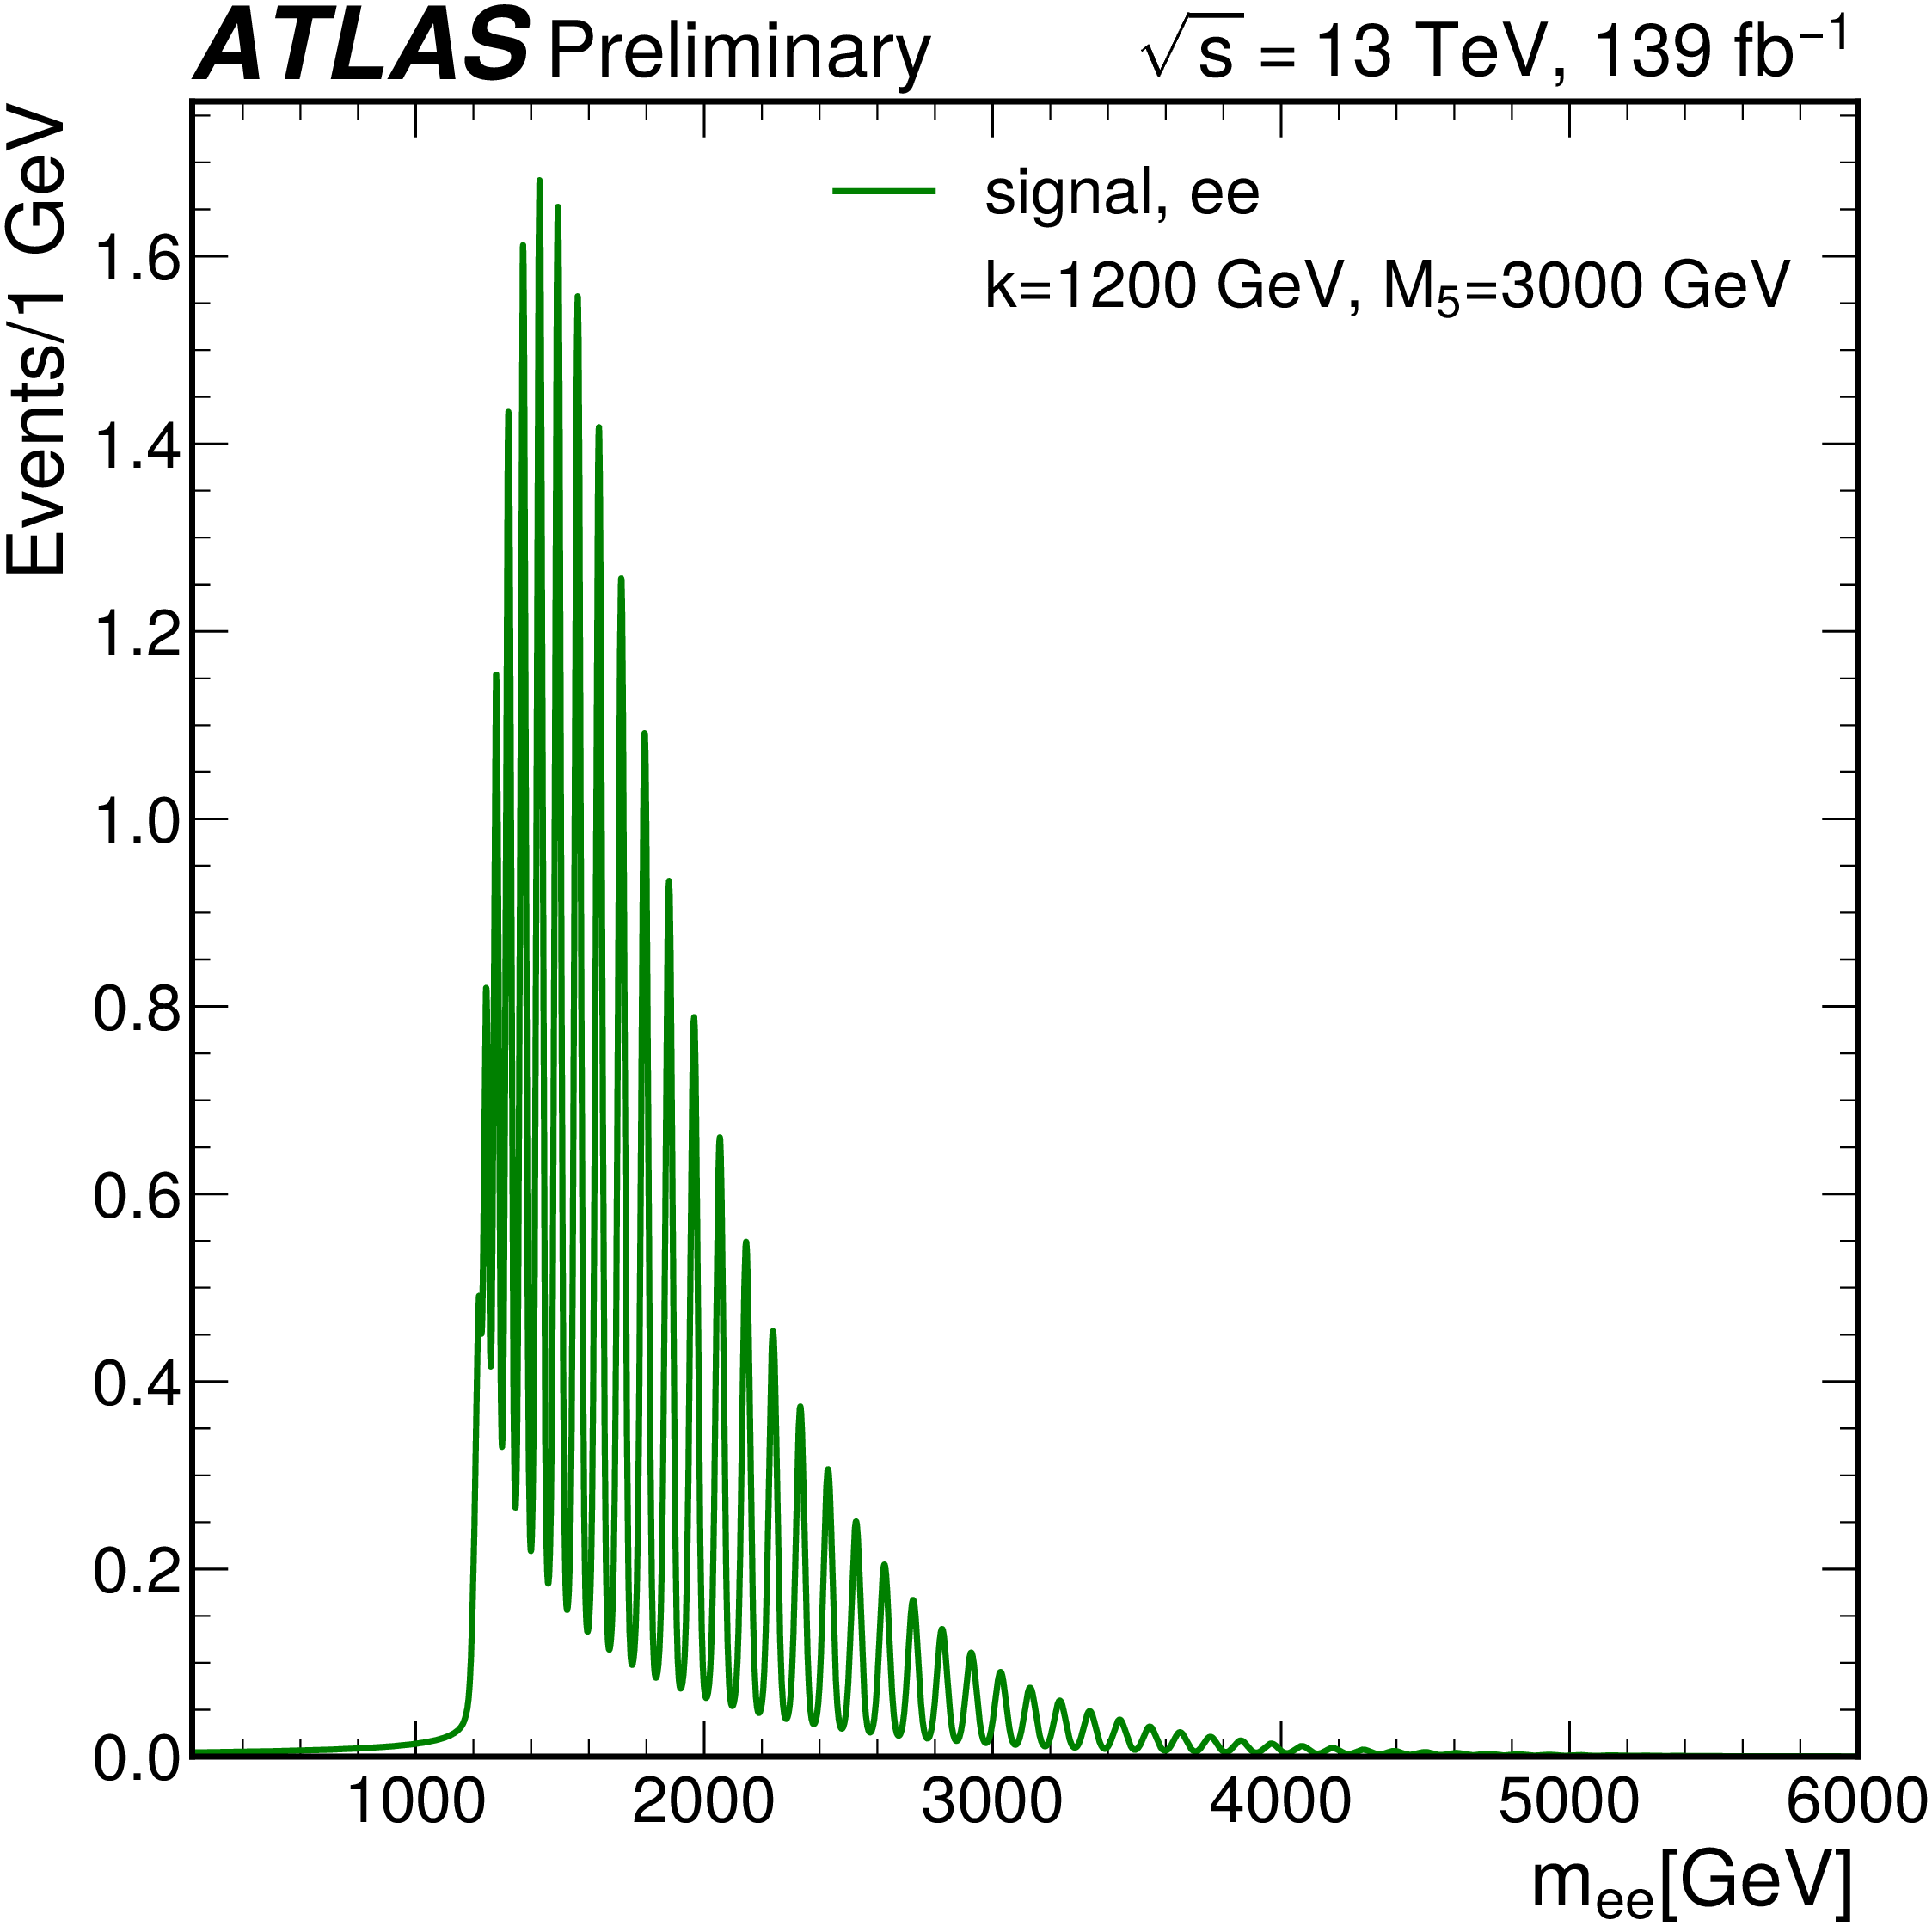
\includegraphics[width=\textwidth]{signal}
         \caption{}
         \label{fig:signal}
     \end{subfigure}
     \begin{subfigure}[b]{0.25\textwidth}
         \centering
         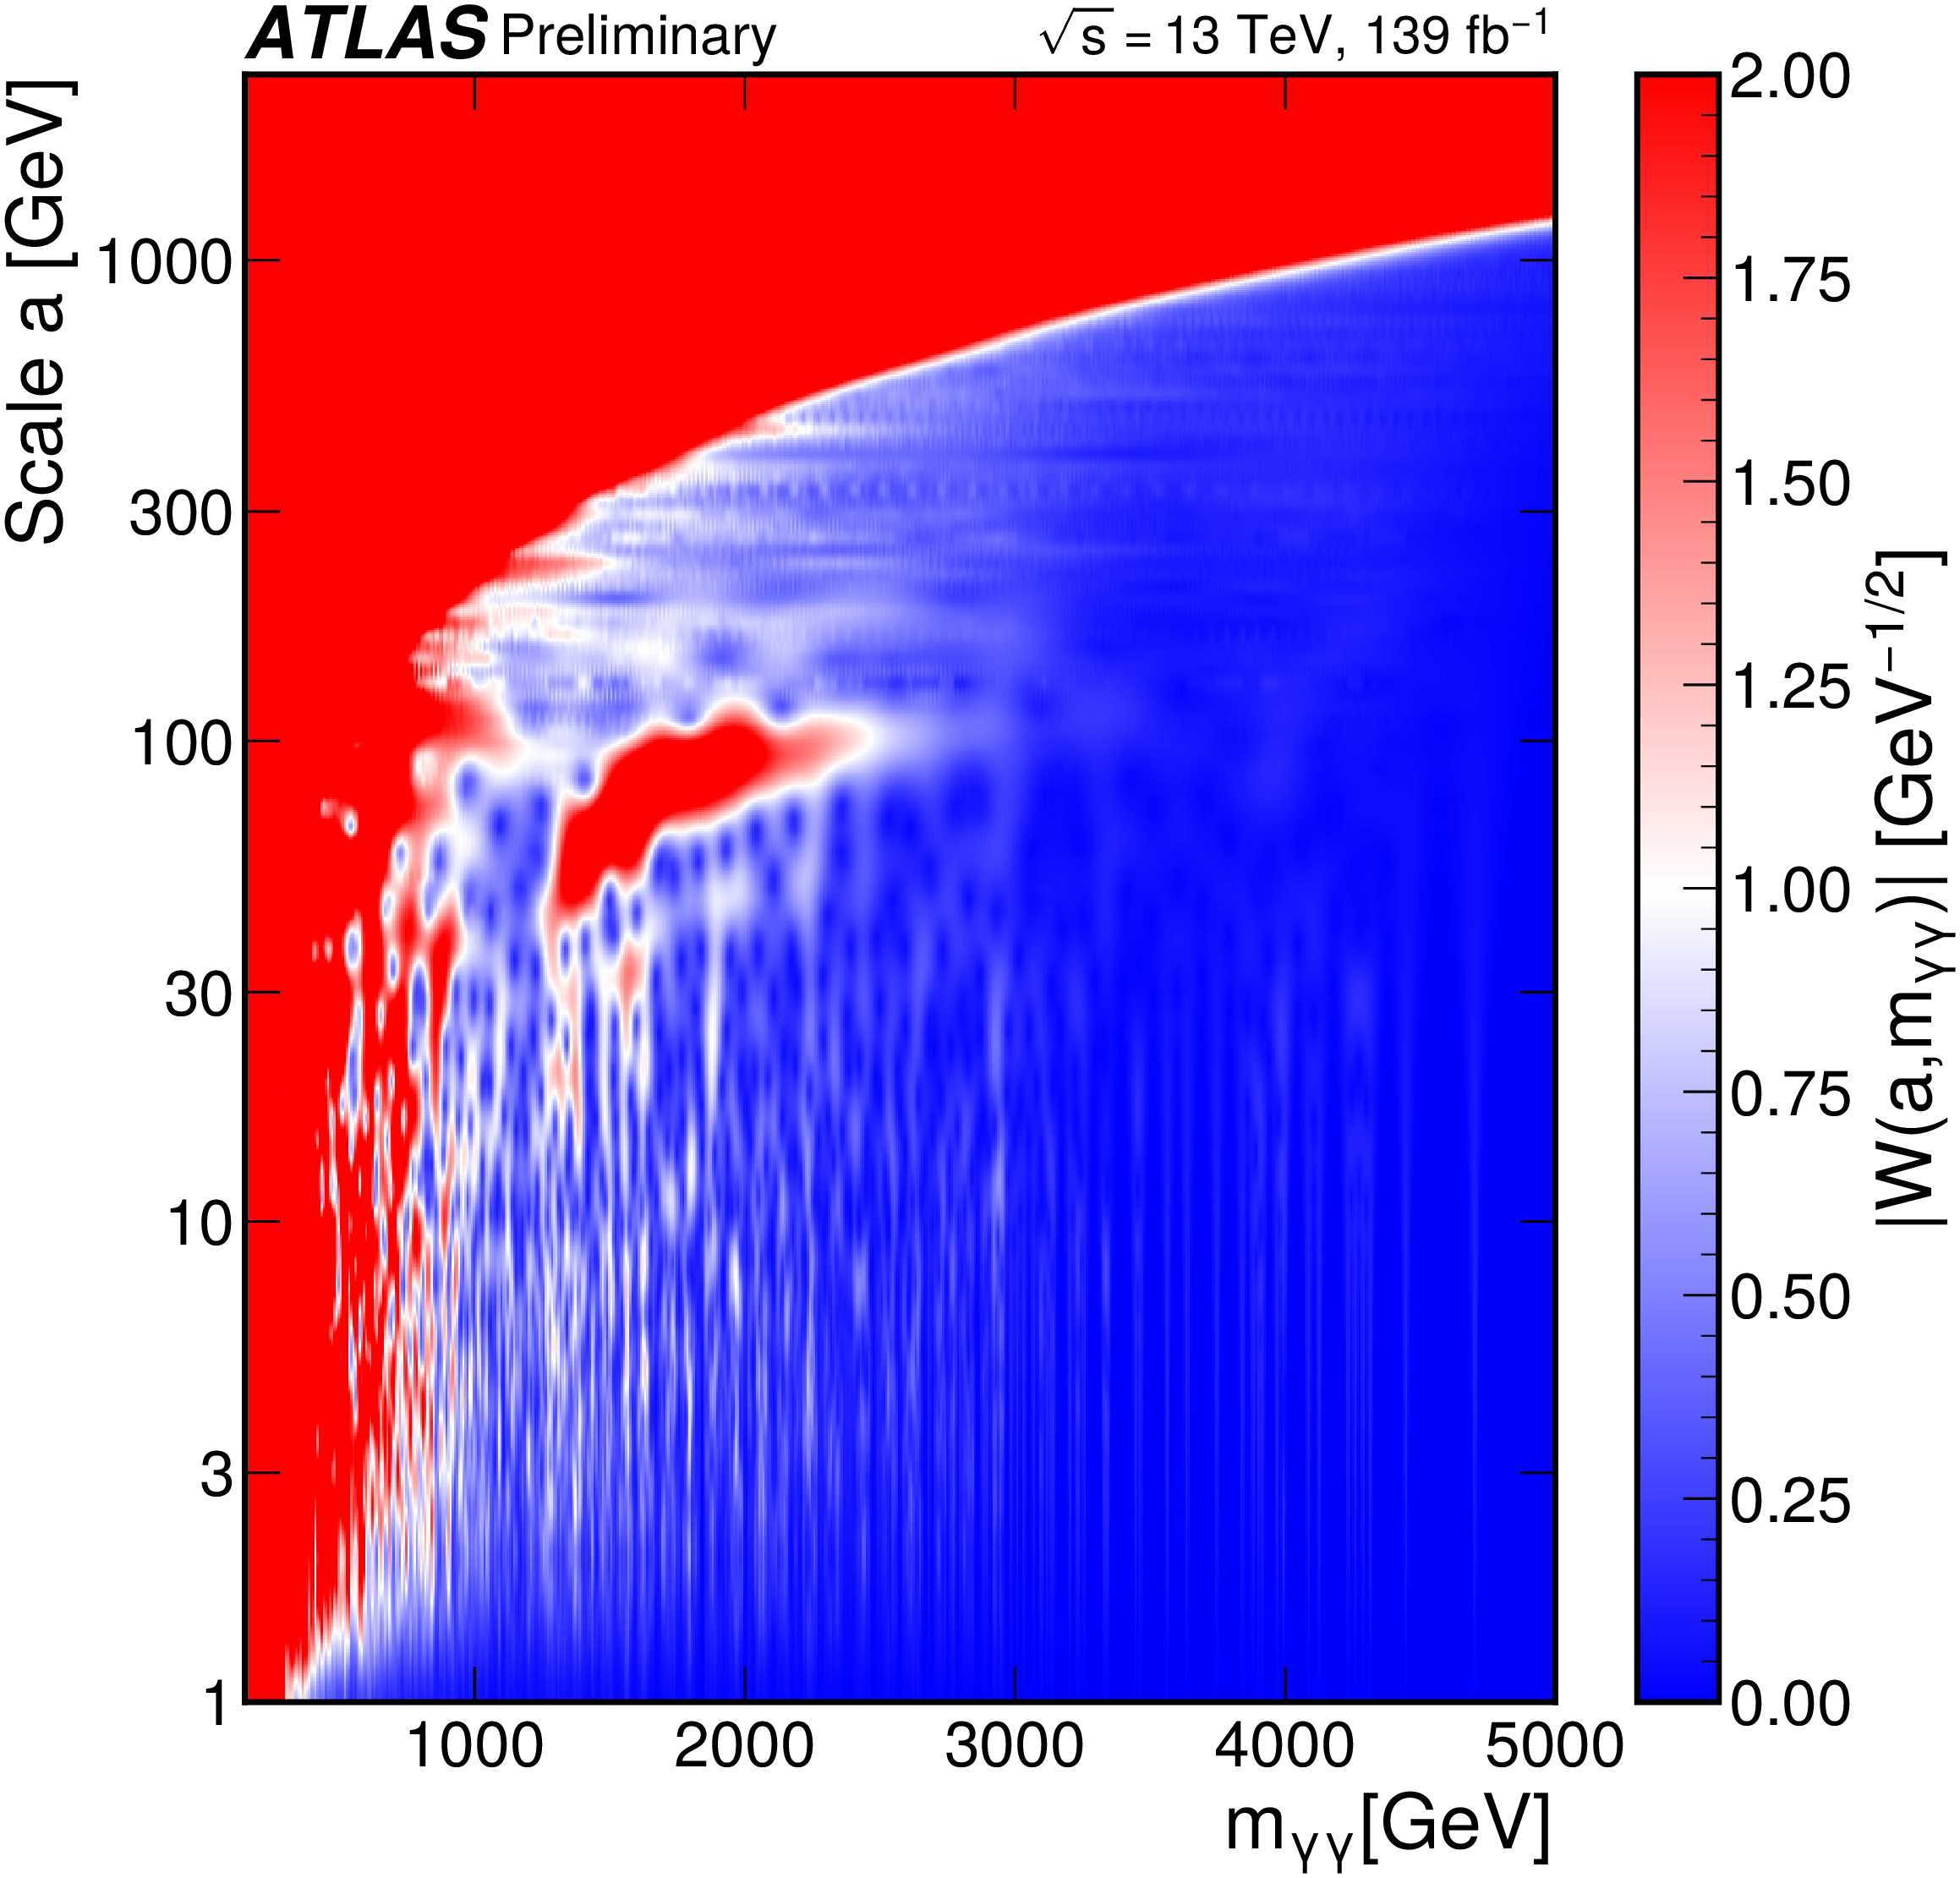
\includegraphics[width=\textwidth]{bkgsig}
         \caption{}
         \label{fig:shape}
     \end{subfigure}
     \begin{subfigure}[b]{0.25\textwidth}
         \centering
         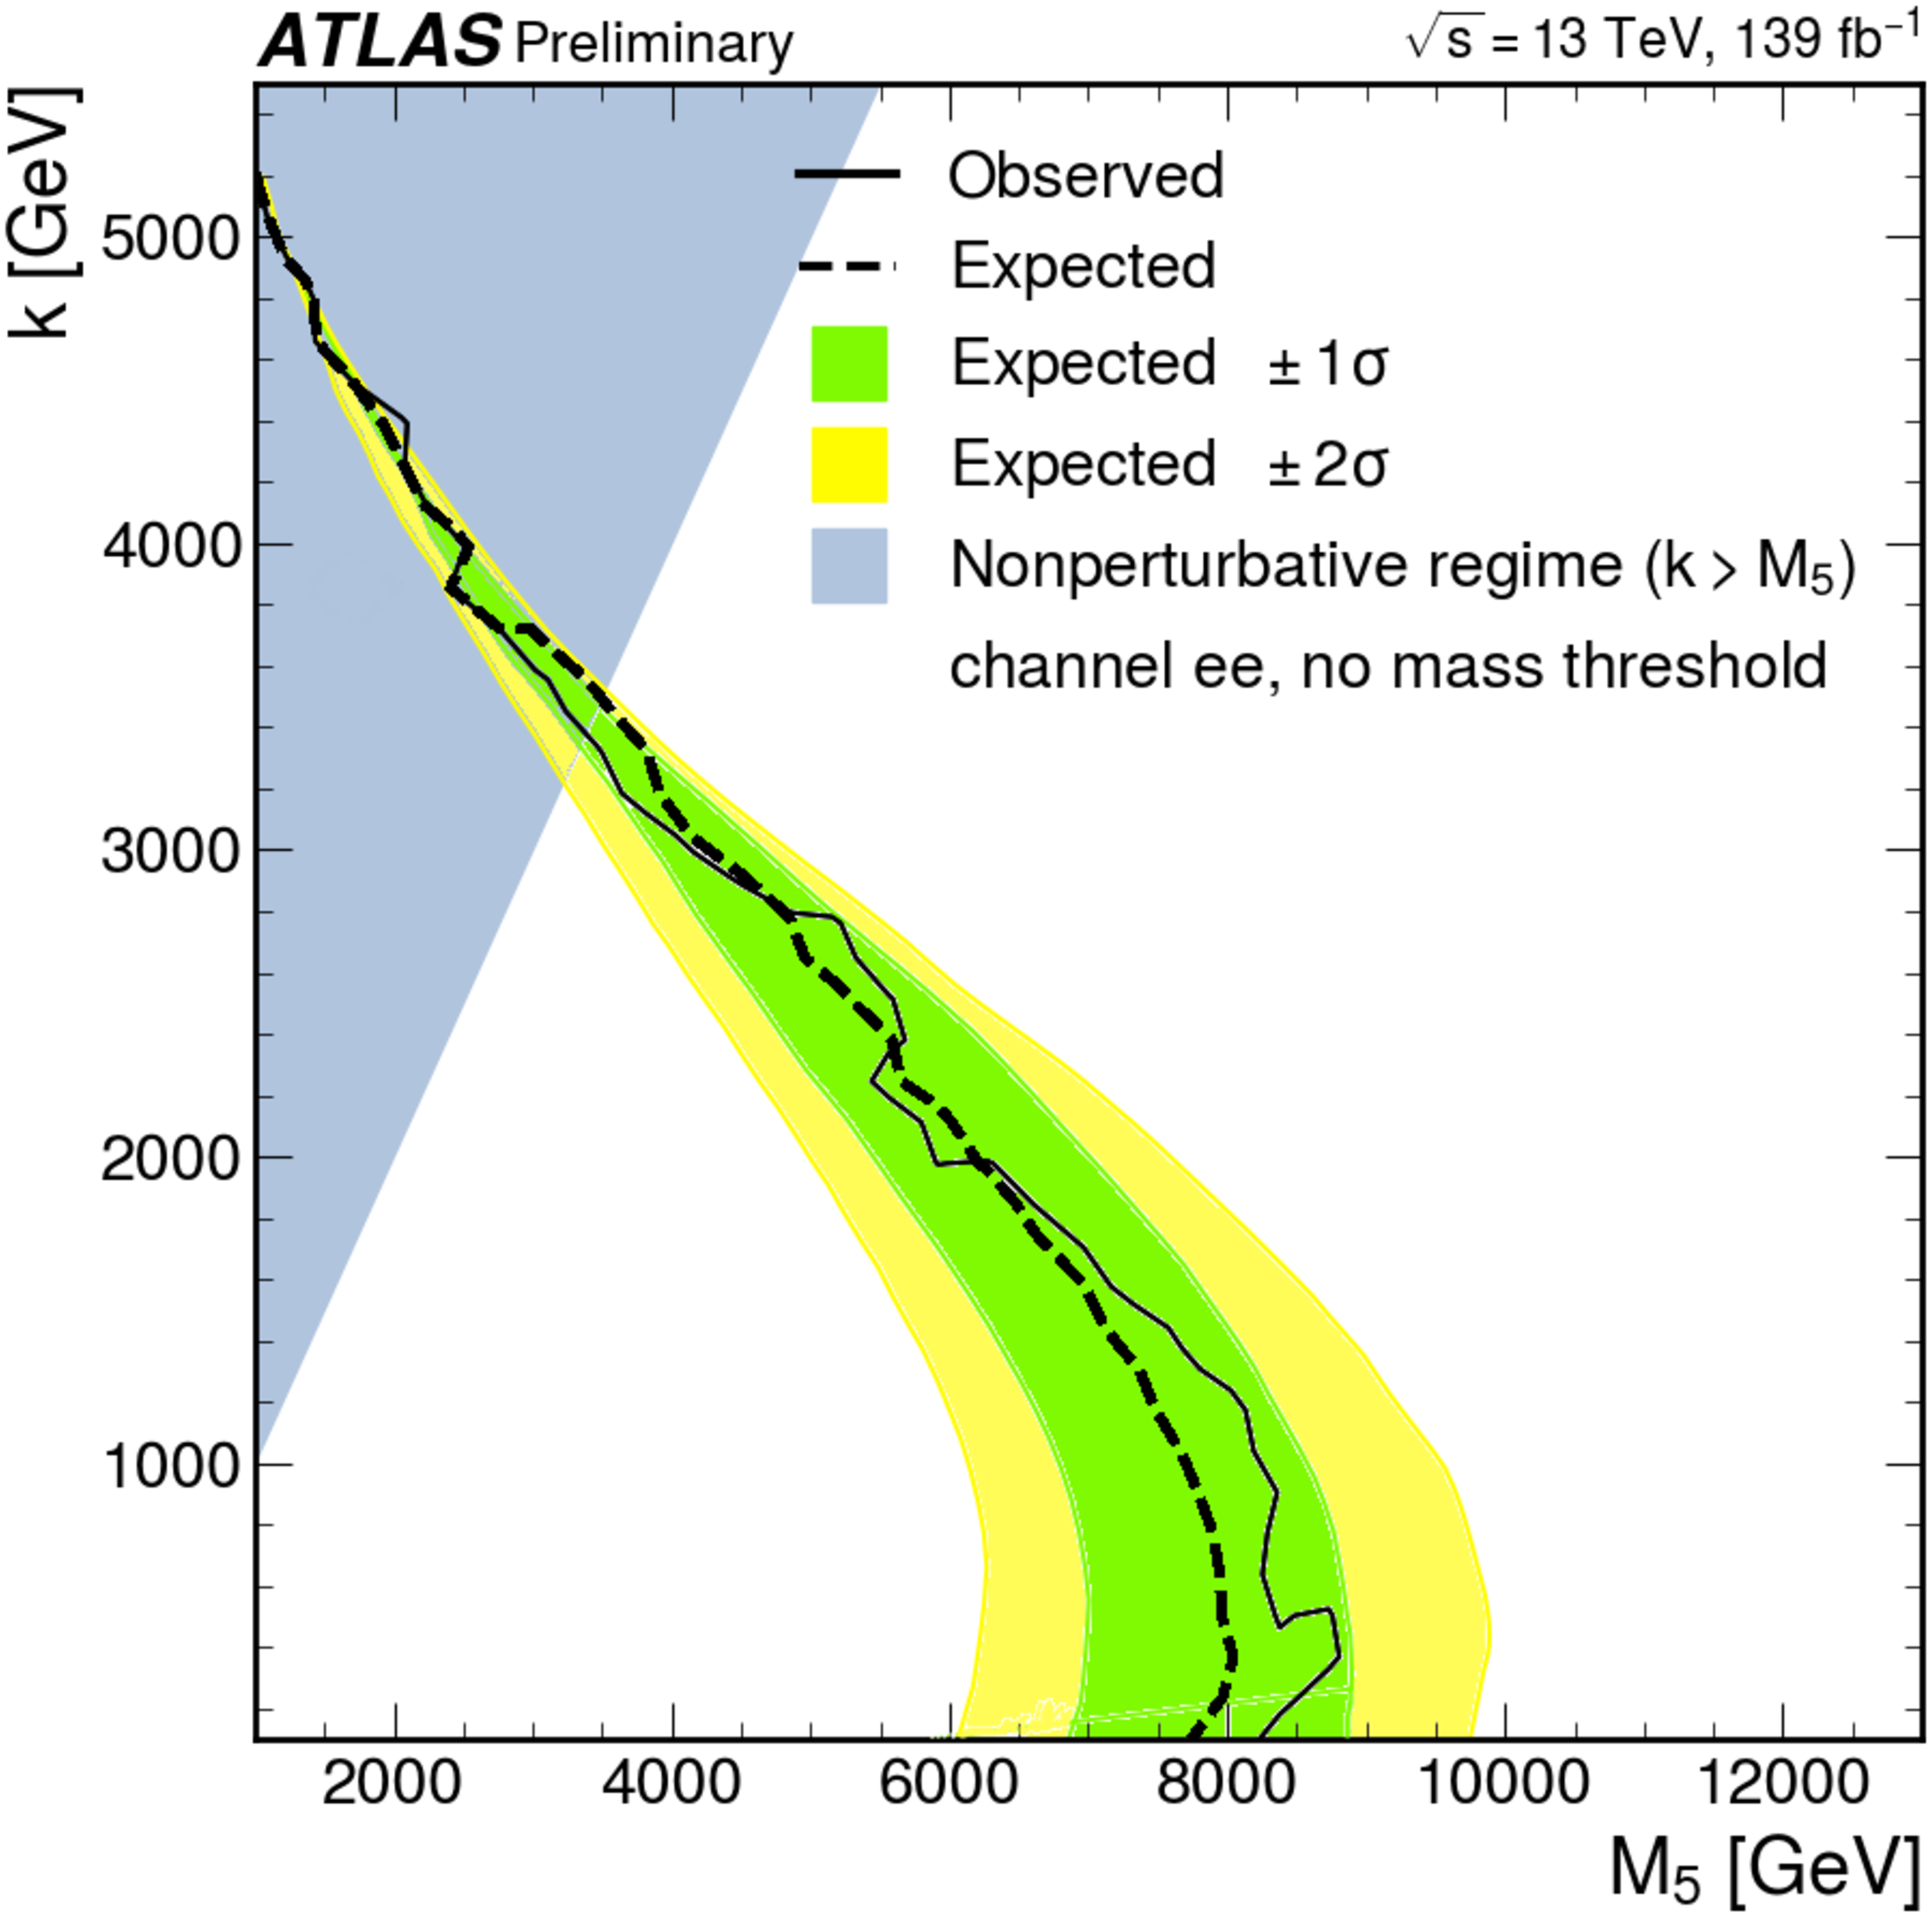
\includegraphics[width=\textwidth]{periodic}
         \caption{}
         \label{fig:perlimits}
     \end{subfigure}
        \caption{(a): The di-electron mass spectrum of a periodic signal. (b): Scalogram of a signal + background sample. (c): Observed (solid line) and expected (dashed line) limits on the model parameters, $M_{5}$ and $k$\protect\cite{period}.}
        \label{fig:periodic}
\end{figure}

\section{Summary}

The search programme at ATLAS is expanding in multiple fronts. Advanced detector
performance and modern analysis techniques allow us to greatly enhance the
sensitivities to a variety of BSM models. The unexplored regions and the gaps
are being filled with new searches applying unique search strategies. Last but
not the least, ATLAS is pioneering brand new signatures that challenge
traditional methods vastly, motivating us to think out of the box and experiment
fresh new methodologies. In addition, more effective theory interpretations are
carried out in precision SM measurements such as the lepton flavour violating
top measurement~\cite{top}. There are many interesting ongoing searches besides
the ones covered in this article, including exciting Run 3 results. More
highlights are coming.       

\section*{References}

\begin{thebibliography}{99}

\bibitem{vlq} The ATLAS Collaboration, ATLAS-CONF-2023-020, http://cds.cern.ch/record/2856892
\bibitem{rhn} The ATLAS Collaboration, CERN-EP-2023-034, https://arxiv.org/abs/2304.09553
\bibitem{tau} The ATLAS Collaboration, CERN-EP-2023-008, https://arxiv.org/abs/2303.09444
\bibitem{bbyy} The ATLAS Collaboration, ATLAS-CONF-2023-009, http://cds.cern.ch/record/2854839
\bibitem{micro} The ATLAS Collaboration, CERN-EP-2023-038, https://arxiv.org/abs/2305.02005
\bibitem{dark} The ATLAS Collaboration, ATLAS-CONF-2023-016, http://cds.cern.ch/record/2855334
\bibitem{tttt} The ATLAS Collaboration, CERN-EP-2023-048, https://arxiv.org/abs/2304.01678
\bibitem{period} The ATLAS Collaboration, CERN-EP-2023-073, https://arxiv.org/abs/2303.09444
\bibitem{top} The ATLAS Collaboration, ATLAS-CONF-2023-001, http://cds.cern.ch/record/2845451

\end{thebibliography}

\end{document}

%%%%%%%%%%%%%%%%%%%%%%
% End of moriond.tex  %
%%%%%%%%%%%%%%%%%%%%%%


%%% Local Variables: 
%%% mode: latex
%%% TeX-master: t
%%% End: 

%%% Local Variables: 
%%% mode: latex
%%% TeX-master: t
%%% End: 

%%% Local Variables: 
%%% mode: latex
%%% TeX-master: t
%%% End: 
